\documentclass[12pt]{article}

\usepackage[margin=1.0in]{geometry}
\usepackage[parfill]{parskip}
\usepackage{amsmath}
\usepackage{amssymb}
\usepackage{amsthm}
\usepackage{algorithm}
\usepackage{algorithmic}
\usepackage{graphicx}
\usepackage[font=bf]{caption}
\usepackage{changepage}
\usepackage{hyperref}



%-------------------------------------------------------------------------------
\begin{document}
%-------------------------------------------------------------------------------



\setlength{\parskip}{12pt}      % set paragraph skipping to one whole line
\setlength{\tabcolsep}{12pt}    % give some room between table columns
\hfuzz=60pt                     % give a little margin room for the double-column tables



% establish a condensed itemized list format
\newenvironment{myitemize}
{ \begin{itemize}
    \setlength{\itemsep}{0pt}
    \setlength{\parskip}{0pt}
    \setlength{\parsep}{0pt}     }
{ \end{itemize}                  } 



% establish theorem and lemma formats
\newtheorem{theorem}{Theorem}[section]
\newtheorem{lemma}[theorem]{Lemma}



\begin{titlepage}
    \begin{center}
        \vspace*{\fill}
        
        \huge
        The Kalman Filter \\
        
        \large
        An Adventure in Derivation
        
        \vspace{24pt}
        
        \large
        Robert S. Huston \\
        Pinpoint Dynamics, LLC \\
        
        \vspace{24pt}
        
        \today
        
        \vspace{24pt}
        
        \large
        Copyright © 2024, 2025 Robert S. Huston. All rights reserved.
        
        \vfill
    \end{center}
\end{titlepage}



\begin{abstract}
This document presents an assorted collection of derivations and notes pertaining to the
Kalman filter. They are targeted to the practicing engineer who has been tasked with
developing and implementing a Kalman filtering solution. The mathematical derivations are
intended to eliminate the mysteries of how and why the Kalman filter works. In addition,
the document presents the various versions of the Kalman filter and offers some key
implementation strategies.
\end{abstract}



\clearpage



\begin{adjustwidth}{1in}{1in}
    \vspace*{\fill}
    
    \textit{
        So I jump ship in Hong Kong and I make my way over to Tibet, and I get on as a
        looper at a course over in the Himalayas.
        A looper, you know, a caddy, a looper, a jock. So, I tell them I'm a pro jock,
        and who do you think they give me? The Dalai Lama, himself. Twelfth son of the Lama.
        The flowing robes, the grace, bald...striking. So, I'm on the first tee with him.
        I give him the driver. He hauls off and whacks one - big hitter, the Lama - long,
        into a ten-thousand foot crevasse, right at the base of this glacier.
        Do you know what the Lama says? "Gunga galunga...gunga, gunga-lagunga."
        So we finish the eighteenth and he's gonna stiff me. And I say, "Hey, Lama, hey,
        how about a little something, you know, for the effort, you know."
        And he says, "Oh, uh, there won't be any money, but when you die, on your deathbed,
        you will receive total consciousness." So I got that goin' for me, which is nice.
    }
    
    - Carl Spackler (Bill Murray, "Caddyshack" - 1980)
    
    \vfill
\end{adjustwidth}



\clearpage



\tableofcontents



\clearpage



\section{Introduction}
\label{Introduction}

Consider the discrete-time linear system dynamical process model and linear observation model

\begin{equation*}
    \begin{aligned}
        \mathbf{x}_{k+1} &= \mathbf{\Phi}_{k+1|k} \mathbf{x}_k + \mathbf{u}_k + \mathbf{\Gamma}_{k+1|k} \mathbf{w}_k \\
        \mathbf{z}_k &= \mathbf{H}_k \mathbf{x}_k + \mathbf{v}_k
    \end{aligned}
\end{equation*}

where $\mathbf{x}$ is an $n \times 1$ state vector,
$\mathbf{\Phi}$ is an $n \times n$ state transition matrix,
$\mathbf{u}$ is an $n \times 1$ control input,
$\mathbf{\Gamma}$ is an $n \times p$ disturbance distribution matrix,
and $\mathbf{w}$ is a $p \times 1$ white process noise sequence of random disturbances with covariance

\begin{equation*}
    \mathbf{Q}_k = E \left\{ \mathbf{w}_k \mathbf{w}_k^T \right\}
\end{equation*}

and where $\mathbf{z}$ is an $m \times 1$ observation vector,
$\mathbf{H}$ is an $m \times n$ observation transformation matrix,
and $\mathbf{v}_k$ is an $m \times 1$ white error noise sequence of random observation errors with covariance

\begin{equation*}
    \mathbf{R}_k = E \left\{ \mathbf{v}_k \mathbf{v}_k^T \right\}
\end{equation*}

and where both the process and observation noise sequences are uncorrelated

\begin{equation*}
    E \left\{ \mathbf{w}_i \mathbf{v}_j^T \right\} = \mathbf{0} \, , \phantom{.} \mathrm{for} \, \mathrm{all} \, i \, \mathrm{and} \, j
\end{equation*}

Figure \ref{fig:dt-linear-system} diagrammatically depicts the linear system model.

\begin{figure}[ht]
    \centering
    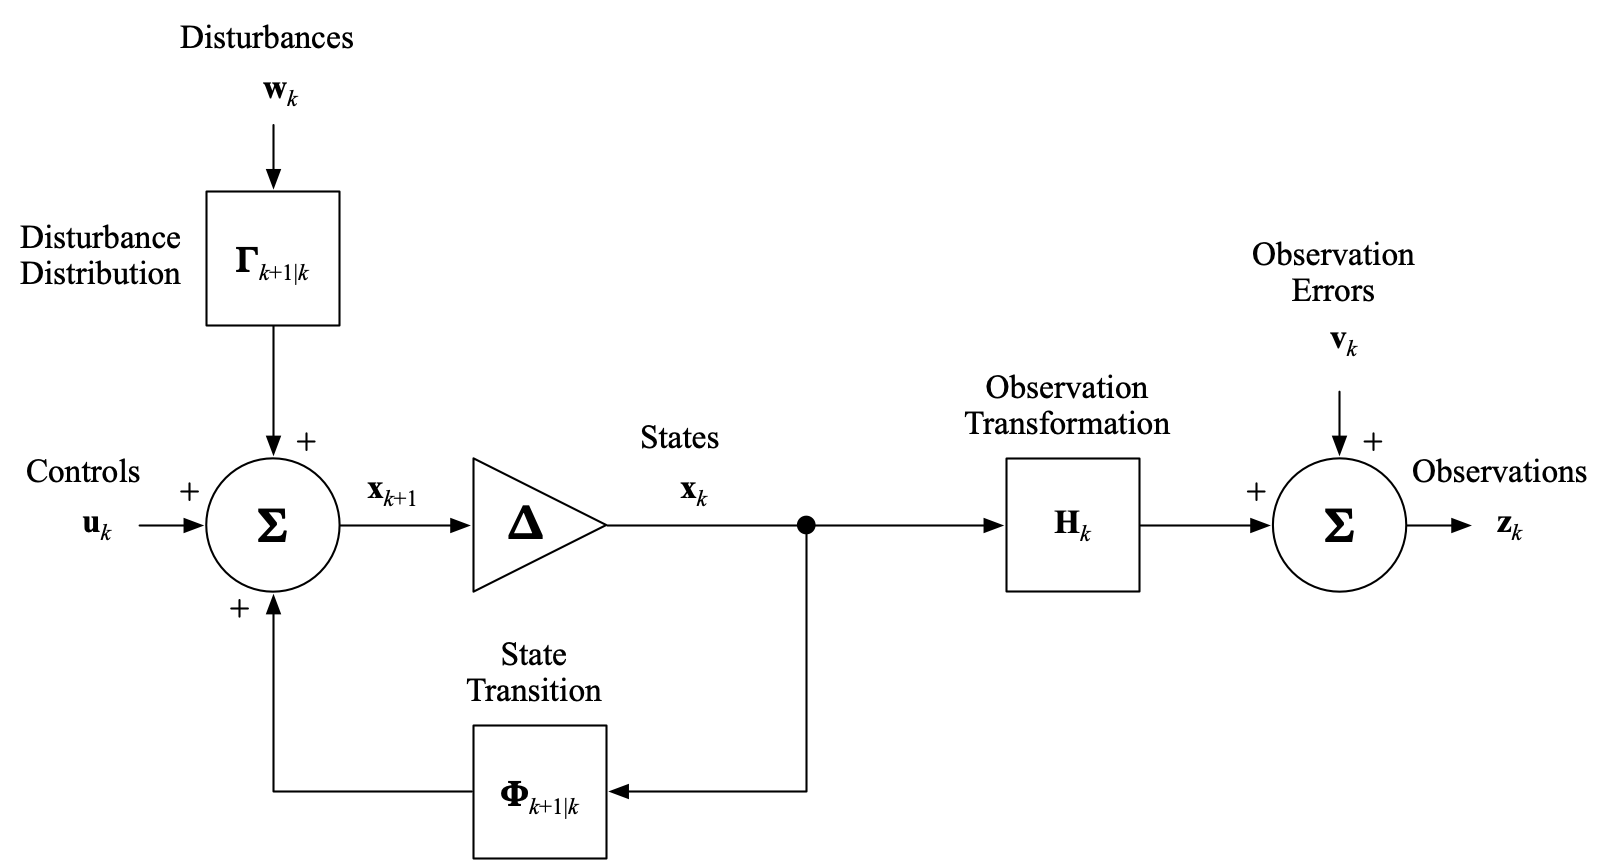
\includegraphics[width=0.95\textwidth]{images/DT-Linear-System.png}
    \caption{Discrete-Time Linear System}
    \label{fig:dt-linear-system}
\end{figure}

Given the observations, $\mathbf{z}_k$,
the modeling knowledge of $\mathbf{\Phi}_{k+1|k}$, $\mathbf{\Gamma}_{k+1|k}$, and $\mathbf{H}_k$,
and the statistical characteristics of $\mathbf{w}_k$ and $\mathbf{v}_k$,
the Kalman filter provides an optimal estimate of the state, $\mathbf{x}_k$, at time event $k$

\begin{equation*}
    \hat{\mathbf{x}}_k = E \left\{ \mathbf{x}_k \right\}
\end{equation*}

with a state estimation error

\begin{equation*}
    \mathbf{e}_k = \mathbf{x}_{k} - \hat{\mathbf{x}}_k
\end{equation*}

and where the covariance of the state estimation error is

\begin{equation*}
    \begin{aligned}
        \mathbf{P}_k &= E \left\{ \mathbf{e}_k \mathbf{e}_k^T \right\} \\
        &= E \left\{ \left[ \mathbf{x}_{k} - \hat{\mathbf{x}}_k \right] \left[ \mathbf{x}_{k} - \hat{\mathbf{x}}_k \right]^T \right\}
    \end{aligned}
\end{equation*}

The well-known Kalman filter \cite{kalman1960} recurrence update cycle is comprised of two steps:
a "projection" or \textit{a priori} update, and a "correction" or \textit{a posteriori} update.

I. Projection (\textit{a priori}) update:

\begingroup
\renewcommand{\arraystretch}{1.25}
\begin{tabular}{l l}
\phantom{.} & $\hat{\mathbf{x}}_{k|k-1} = \mathbf{\Phi}_{k|k-1} \hat{\mathbf{x}}_{k-1} + \mathbf{u}_{k-1}$ \\
\phantom{.} & $\mathbf{P}_{k|k-1} = \mathbf{\Phi}_{k|k-1} \mathbf{P}_{k-1} \mathbf{\Phi}_{k|k-1}^T + \mathbf{\Gamma}_{k|k-1} \mathbf{Q}_{k-1} \mathbf{\Gamma}_{k|k-1}^T$
\end{tabular}
\endgroup

II. Correction (\textit{a posteriori}) update:

\begingroup
\renewcommand{\arraystretch}{1.25}
\begin{tabular}{l l}
\phantom{.} & $\hat{\mathbf{z}}_k = \mathbf{H}_k \hat{\mathbf{x}}_{k|k-1}$ \\
\phantom{.} & $\tilde{\mathbf{z}}_k = \mathbf{z}_k - \hat{\mathbf{z}}_k$ \\
\phantom{.} & $\mathbf{S}_k = \mathbf{H}_k \mathbf{P}_{k|k-1} \mathbf{H}_k^T + \mathbf{R}_k$ \\
\phantom{.} & $\mathbf{K}_k = \mathbf{P}_{k|k-1} \mathbf{H}_{k}^T \mathbf{S}_k^{-1}$ \\
\phantom{.} & $\hat{\mathbf{x}}_k = \hat{\mathbf{x}}_{k|k-1} +\mathbf{K}_k \tilde{\mathbf{z}}_k$ \\
\phantom{.} & $\mathbf{P}_k = \left[ \mathbf{I} - \mathbf{K}_k \mathbf{H}_k \right] \mathbf{P}_{k|k-1}$
\end{tabular}
\endgroup

Figure \ref{fig:kf-diagram} diagrammatically depicts the Kalman filter.

\begin{figure}[ht]
    \centering
    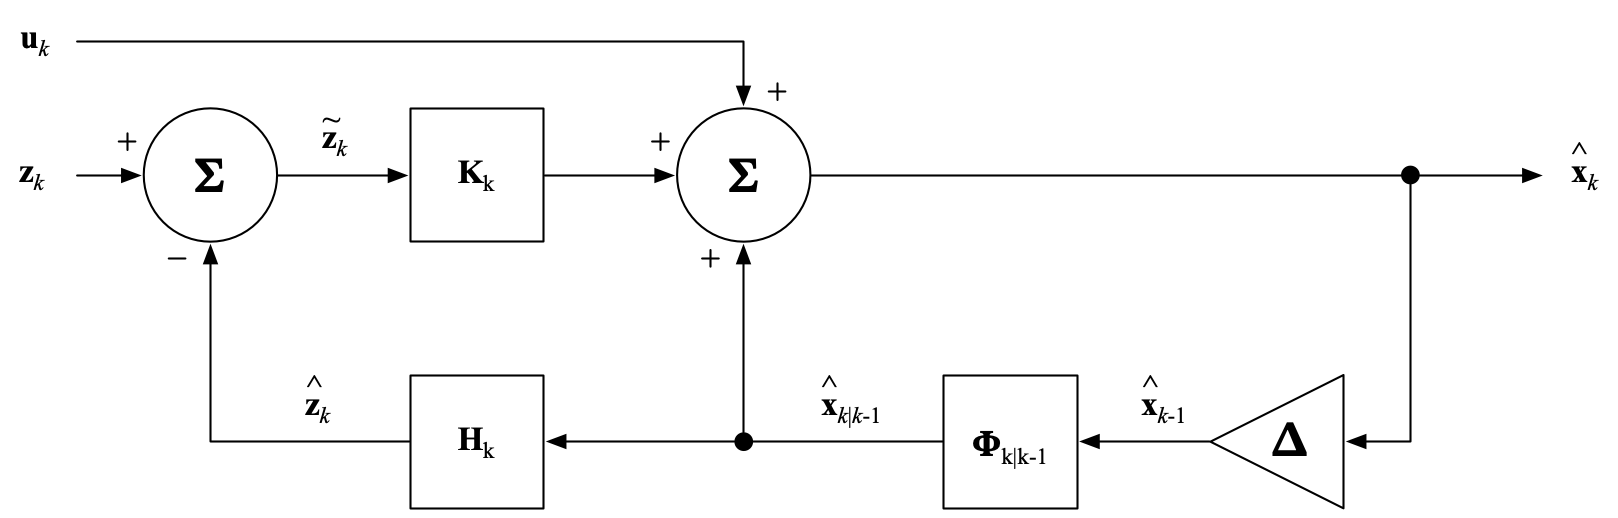
\includegraphics[width=0.95\textwidth]{images/KF-Diagram.png}
    \caption{Kalman Filter Diagram}
    \label{fig:kf-diagram}
\end{figure}

Unfortunately, the vast literature for the Kalman filter, and its varieties, can be
overwhelmingly confounding. Different variables are used. Different notations are used.
Different terms are used. The complexity of some of the mathematical proofs and theorems
can obscure the more important matters.

And then there are questions \ldots many questions.
What’s with all these equations?
What makes them so special?
Where do they come from?
What is meant by "optimal" gain?
Why can’t I just use least-squares estimation?
Isn’t the Kalman filter just a specialized least-squares filter anyway?
What does it mean when it is said that "$\mathbf{S}_k$" represents the covariance of the observation error?
Why are there so many different forms of the filter, and which one should I use?
And did Jeffrey Epstein really kill himself?

This document is an assorted collection of derivations and notes pertaining to the Kalman
filter. They are targeted to the practicing engineer who has been tasked with developing
and implementing a Kalman filtering solution. The mathematical derivations are therefore
intended to eliminate some of the mysteries of how and why the Kalman filter works, as
well as what the various versions and implementation strategies have to offer.

Some assumptions are made about the reader:

\begin{myitemize}
    \item The reader understands basic matrix algebra
    \item The reader understands basic calculus
    \item The reader understands basic probability and statistics
\end{myitemize}

Lastly, this document is written the the way I wished I could have experienced when I was
first learning the Kalman filter. Hopefully, it is helpful to the reader as is.
If not, well then too bad.

\clearpage

\section{Conventions and Notations}
\label{Conventions and Notations}

When I began my journey into studying the Kalman filter, my primary reference was the
"Robert Grover Brown" book \cite{rgbrown1983}, and much of my choice of conventions and
notations comes from that book. I also heavily relied on Sorenson’s material
\cite{sorenson1985} which was consistent with R.G. Brown notation. As I accumulated other
references over the years, I discovered that the Brown/Sorenson conventions and notations
were dominant. Granted there are other conventions and notations in the Kalman filtering
literature, but I feel most at home when using the Brown/Sorenson conventions and notations,
and those are the ones I’ve chosen to adopt in this document.

In particular, $\mathbf{x}_k$ represents a system state vector at time event "$k$",
$\mathbf{\Phi}_{k+1|k}$ represents a linear state transition matrix that transitions the
state from time events "$k$" to "$k+1$",
$\mathbf{z}_k$ represents an observation (i.e., measurement) vector that observes the
system output at time event "$k$",
and $\mathbf{H}_k$ represents a linear observation transformation from $\mathbf{x}_k$
to $\mathbf{z}_k$.
Additionally, $\mathbf{w}_k$ and $\mathbf{v}_k$ represent random sequences that model the
system dynamics variations and observation variations, respectively, with covariances
$\mathbf{Q}_k$ and $\mathbf{R}_k$, respectively.
Lastly, the system state estimation error covariance is represented by $\mathbf{P}_k$.

In addition to the many different choices of variables in the technical literature, there
are also many notational styles.
For instance, instead of using the "$k$" and "$k+1|k$" subscripts, some references use
functional forms instead, as in "$\mathbf{x}(k)$" and "$\mathbf{\Phi}(k+1|k)$".
Others use "$+$" and "$-$" indicators to differentiate \textit{a priori} variables from
\textit{a posteriori} variables, e.g., $\mathbf{P}_k^-$ instead of $\mathbf{P}_{k|k-1}$,
and $\mathbf{P}_k^+$ instead of $\mathbf{P}_{k|k}$.
The notations adopted in this document strive to make the equations clear (or as clear
as they can be) without being "too busy" in the variable descriptors;
$\mathbf{\Phi}_{k+1|k}$ is more readable in an expression than $\mathbf{\Phi}(k+1|k)$.

There are many references that do not distinguish visually between a scalar quantity and
a matrix quantity. While this may have been a necessity in the days of typewriters and
early word processors, it also does the reader an extreme disservice. Knowing that a
variable is a scalar or a matrix is fundamental in the understanding of an equation or
derivation, and given today’s technology in word processing and electronic typesetting,
there is no excuse for not adhering to the accepted conventions where an italic variable,
$s$, is a scalar quantity, and a boldface variable, $\mathbf{M}$, is a matrix quantity.

I’ve often wondered why this particular choice of variables was picked by certain authors.
For instance, why use $\mathbf{z}$ for the observation vector when the state vector is
$\mathbf{x}$ and the natural choice would be to use $\mathbf{y}$ instead? After all,
that’s what all the classical linear control system theory resources use. And why use
$\mathbf{H}$ as the linear observation transformation instead of something more consistent
with classical linear control system theory? My uneducated guess is that using $\mathbf{z}$
allows for the use of $\mathbf{y}$ to represent additional state values (e.g., hidden
states) in augmented system formulations, and using $\mathbf{H}$ is simply a natural
alphabetic progression after $\mathbf{F}$ and $\mathbf{G}$ are assigned for discrete-time
system functional transformations. For instance, consider the classical continuous-time
linear system description:

\begin{equation*}
    \begin{aligned}
        \mathbf{\dot{x}} &= \mathbf{A} \mathbf{x} + \mathbf{B} \mathbf{u} \\
        \mathbf{y} &= \mathbf{C} \mathbf{x} + \mathbf{D} \mathbf{u} \\
    \end{aligned}
\end{equation*}

where $\mathbf{x}$ is the system state, $\mathbf{u}$ is the control input, and $\mathbf{y}$
is the output observation. In transforming to a discrete-time description, a natural
choice of variables would be

\begin{equation*}
    \begin{aligned}
        \mathbf{x}_{k+1} &= \mathbf{F}_k \mathbf{x}_k + \mathbf{G}_k \mathbf{u}_k \\
        \mathbf{z}_k &= \mathbf{H}_k \mathbf{x}_k + \mathbf{J}_k \mathbf{u}_k
    \end{aligned}
\end{equation*}

We should stay away from using $\mathbf{E}$ because it could easily be confused with the
expectation operation $E \left\{ \cdots \right\}$, and we can’t use $\mathbf{I}$ because
that’s the identity matrix (although I’ve seen some authors use $\mathbf{I}_k$ to represent
an information matrix value at time event "$k$", causing me horrible confusion), so the
choices of $\mathbf{H}$ seems to make logical sense. Similarly, the choices for covariance
values appear to be alphabetically assigned. If $\mathbf{P}$ is our first-assigned covariance,
then using $\mathbf{Q}$ and $\mathbf{R}$ make sense for the next two assignments. Of course,
this reasoning behind the assignments is pure conjecture on my part, but it allows me to
find order in the conventions that I’ve chosen from R.G. Brown and others.

The following list summarizes the general conventions and notations used in this document:

\begin{myitemize}
    \item An italic variable, $s$, designates a scalar quantity (the variable can be of any case)
    \item A boldface lower-case variable, $\mathbf{v}$, designates a vector matrix quantity
    \item A boldface upper-case variable, $\mathbf{M}$, designates a block matrix quantity
    \item $\mathbf{x}_k$ designates a system state vector at time event "$k$"
    \item $\hat{\mathbf{x}}_k$ designates an estimate of the system state vector, $\mathbf{x}_k$, at time event "$k$"
    \item $\mathbf{P}_k$ designates the covariance matrix of the state estimation error, $\mathbf{x}_k - \hat{\mathbf{x}}_k$
    \item $\mathbf{\Phi}_{k+1|k}$ designates a linear state transition matrix that transitions $\mathbf{x}_k$ from time events "$k$" to "$k+1$"
    \item $\mathbf{u}_k$ designates a system control input vector at time event "$k$"
    \item $\mathbf{w}_k$ designates a system process random variation vector at time event "$k$"
    \item $\mathbf{Q}_k$ designates the covariance matrix of the system process random variation, $\mathbf{w}_k$
    \item $\mathbf{\Gamma}_{k+1|k}$ designates a linear matrix that transforms $\mathbf{w}_k$ from time events "$k$" to "$k+1$" into the state space of $\mathbf{x}_k$
    \item $\mathbf{z}_k$ designates an observation (i.e., measurement) vector that observes the system at time event "$k$"
    \item $\hat{\mathbf{z}}_k$ designates an estimate of the observation vector, $\mathbf{z}_k$, at time event "$k$"
    \item $\mathbf{R}_k$ designates the covariance matrix of the observation estimation error, $\mathbf{z}_k - \hat{\mathbf{z}}_k$
    \item $\mathbf{H}_k$ designates a linear observation transformation matrix from the state space of $\mathbf{x}_k$ into the state space of $\mathbf{z}_k$
    \item $\mathbf{v}_k$ designates an observation random variation vector at time event "$k$"
    \item $\mathbf{R}_k$ designates the covariance matrix of the observation random variation, $\mathbf{v}_k$
    \item $\mathbf{K}_k$ designates the state estimation filter gain matrix, i.e., the Kalman gain
\end{myitemize}

\clearpage

\section{Weighted Least-Squares Estimation}
\label{Weighted Least-Squares Estimation}

Consider the overdetermined observation system

\begin{equation*}
    \mathbf{z} = \mathbf{H} \mathbf{x} + \mathbf{v}
\end{equation*}

where $\mathbf{z}$ is an $m \times 1$ observation vector,
$\mathbf{x}$ is an $m \times 1$ state vector,
$\mathbf{H}$ is an $m \times n$ observation matrix,
and $\mathbf{v}$ is an $m \times 1$ random vector of observation errors with covariance

\begin{equation*}
    E \left\{ \mathbf{v} \mathbf{v}^T \right\} = \mathbf{R}
\end{equation*}

As stated previously, $m \ge n$, i.e., there can be more observations than there are states.
So $\mathbf{H}$ is not necessarily square:

\begin{equation*}
    \begin{bmatrix}
    z_1 \\
    z_2 \\
    z_3 \\
    z_4 \\
    z_5 \\
    \vdots \\
    z_m
    \end{bmatrix}
    =
    \begin{bmatrix}
    h_{11} & h_{12} & h_{13} & \dots & h_{1n} \\
    h_{21} & h_{22} & h_{23} & \dots & h_{2n} \\
    h_{31} & h_{32} & h_{33} & \dots & h_{3n} \\
    h_{41} & h_{42} & h_{43} & \dots & h_{4n} \\
    h_{51} & h_{52} & h_{53} & \dots & h_{5n} \\
    \vdots & \vdots & \vdots & \ddots & \vdots \\
    h_{m1} & h_{m2} & h_{m3} & \dots & h_{mn}
    \end{bmatrix}
    \begin{bmatrix}
    x_1 \\
    x_2 \\
    x_3 \\
    \vdots \\
    x_n
    \end{bmatrix}
    +
    \begin{bmatrix}
    v_1 \\
    v_2 \\
    v_3 \\
    v_4 \\
    v_5 \\
    \vdots \\
    v_m
    \end{bmatrix}
\end{equation*}

Assume that we already have a state estimate, $\hat{\mathbf{x}}$. We can then determine the
corresponding observation estimate, $\hat{\mathbf{z}}$, from

\begin{equation*}
    \hat{\mathbf{z}} = \mathbf{H} \hat{\mathbf{x}}
\end{equation*}

We form the observation residual, i.e., the observation error

\begin{equation*}
    \tilde{\mathbf{z}} = \mathbf{z} - \hat{\mathbf{z}}
\end{equation*}

We can then form the weighted squared error term

\begin{equation*}
    \epsilon^2 = \tilde{\mathbf{z}}^T \mathbf{W} \tilde{\mathbf{z}}
\end{equation*}

where $\mathbf{W}$ is an arbitrary symmetric weighting matrix.

The objective is to determine the "best" value for $\hat{\mathbf{x}}$ that fits the
observation data $\mathbf{z}$. We will define "best" to be the value of $\hat{\mathbf{x}}$
that minimizes $\epsilon^2$. In other words, we want to find the "least-squares"
estimate of $\mathbf{x}$.

Expanding the terms of $\epsilon^2$ gives

\begin{equation*}
    \begin{aligned}
        \epsilon^2 &= \tilde{\mathbf{z}}^T \mathbf{W} \tilde{\mathbf{z}} \\
                   &= \left[ \mathbf{z} - \hat{\mathbf{z}} \right]^T \mathbf{W} \left[ \mathbf{z} - \hat{\mathbf{z}} \right] \\
                   &= \left[ \mathbf{z} - \mathbf{H} \hat{\mathbf{x}} \right]^T \mathbf{W} \left[ \mathbf{z} - \mathbf{H} \hat{\mathbf{x}} \right] \\
                   &= \left[ \mathbf{z}^T - \hat{\mathbf{x}}^T \mathbf{H}^T \right] \mathbf{W} \left[ \mathbf{z} - \mathbf{H} \hat{\mathbf{x}} \right] \\
                   &= \mathbf{z}^T \mathbf{W} \mathbf{z} - \hat{\mathbf{x}}^T \mathbf{H}^T \mathbf{W} \mathbf{z}
                      - \mathbf{z}^T \mathbf{W} \mathbf{H} \hat{\mathbf{x}} + \hat{\mathbf{x}}^T \mathbf{H}^T \mathbf{W} \mathbf{H} \hat{\mathbf{x}}
    \end{aligned}
\end{equation*}

To find the value of $\hat{\mathbf{x}}$ that minimizes $\epsilon^2$, we differentiate 
$\epsilon^2$ with respect to $\hat{\mathbf{x}}$ and set the resulting expression to zero.
We can make use of the following differentiation formulas:

\begin{equation*}
    \frac{ d \left( \mathbf{a}^T \mathbf{x} \right) }{d \mathbf{x}} = \frac{ d \left( \mathbf{x}^T \mathbf{a} \right) }{d \mathbf{x}} = \mathbf{a}
\end{equation*}

\begin{equation*}
    \frac{ d \left( \mathbf{x}^T \mathbf{A} \mathbf{x} \right) }{d \mathbf{x}} = 2 \mathbf{A} \mathbf{x} \, , \phantom{X} (\mathbf{A} \, \mathrm{is} \, \mathrm{symmetric})
\end{equation*}

We use the differential operation where, if $s$ is a scalar value and $\mathbf{x}$ is a
column vector value, then

\begin{equation*}
    \frac {d s} {d \mathbf{x}} \triangleq
    \begin{bmatrix}
    \dfrac{\partial s}{\partial x_{1}} \\
    \phantom{.} \\
    \dfrac{\partial s}{\partial x_{2}} \\
    \phantom{.} \\
    \dfrac{\partial s}{\partial x_{3}} \\
    \phantom{.} \\
    \vdots
    \end{bmatrix}
\end{equation*}

Then

\begin{equation*}
    \begin{aligned}
        \frac{ d \left( \epsilon^2 \right) }{d \hat{\mathbf{x}}}
        &= - \mathbf{H}^T \mathbf{W} \mathbf{z}
           - \left( \mathbf{z}^T \mathbf{W} \mathbf{H} \right)^T
           + 2 \mathbf{H}^T \mathbf{W} \mathbf{H} \hat{\mathbf{x}} \\
        &= \mathbf{0}
    \end{aligned}
\end{equation*}

and so, observing that $\mathbf{H}^T \mathbf{W} \mathbf{H}$ is invertible, we see that

\begin{equation*}
    \begin{aligned}
        - \mathbf{H}^T \mathbf{W} \mathbf{z}
        -  \left( \mathbf{z}^T \mathbf{W} \mathbf{H} \right)^T
        + 2 \mathbf{H}^T \mathbf{W} \mathbf{H} \hat{\mathbf{x}}
        &= \mathbf{0} \\
        - \mathbf{H}^T \mathbf{W} \mathbf{z}
        - \mathbf{H}^T \mathbf{W} \mathbf{z}
        + 2 \mathbf{H}^T \mathbf{W} \mathbf{H} \hat{\mathbf{x}}
        &= \mathbf{0} \\
        - 2 \mathbf{H}^T \mathbf{W} \mathbf{z}
        + 2 \mathbf{H}^T \mathbf{W} \mathbf{H} \hat{\mathbf{x}}
        &= \mathbf{0} \\
        \mathbf{H}^T \mathbf{W} \mathbf{H} \hat{\mathbf{x}} &= \mathbf{H}^T \mathbf{W} \mathbf{z} \\
        \hat{\mathbf{x}} &= \left( \mathbf{H}^T \mathbf{W} \mathbf{H} \right)^{-1} \mathbf{H}^T \mathbf{W} \mathbf{z} \\
    \end{aligned}
\end{equation*}

Hence the "best" value of $\hat{\mathbf{x}}$ that fits the observation data $\mathbf{z}$
in the least-squares sense is

\boxed{
\parbox{\textwidth}{
\begin{equation}
    \hat{\mathbf{x}} = \left( \mathbf{H}^T \mathbf{W} \mathbf{H} \right)^{-1} \mathbf{H}^T \mathbf{W} \mathbf{z}
\end{equation}
}
}

To find the optimal value of $\mathbf{W}$, we form the state estimation error

\begin{equation*}
    \begin{aligned}
        \mathbf{e} &= \mathbf{x} - \hat{\mathbf{x}} \\
        &= \mathbf{x} - \left( \mathbf{H}^T \mathbf{W} \mathbf{H} \right)^{-1} \mathbf{H}^T \mathbf{W} \mathbf{z} \\
        &= \mathbf{x} - \left( \mathbf{H}^T \mathbf{W} \mathbf{H} \right)^{-1} \mathbf{H}^T \mathbf{W} \left[ \mathbf{H} \mathbf{x} + \mathbf{v} \right] \\
        &= \mathbf{x}
           - \left( \mathbf{H}^T \mathbf{W} \mathbf{H} \right)^{-1} \mathbf{H}^T \mathbf{W} \mathbf{H} \mathbf{x}
           - \left( \mathbf{H}^T \mathbf{W} \mathbf{H} \right)^{-1} \mathbf{H}^T \mathbf{W} \mathbf{v} \\
        &= \mathbf{x} - \mathbf{x}
           - \left( \mathbf{H}^T \mathbf{W} \mathbf{H} \right)^{-1} \mathbf{H}^T \mathbf{W} \mathbf{v} \\
        &= - \left( \mathbf{H}^T \mathbf{W} \mathbf{H} \right)^{-1} \mathbf{H}^T \mathbf{W} \mathbf{v} \\
    \end{aligned}
\end{equation*}

Then the covariance of the state estimation error is

\begin{equation*}
    \begin{aligned}
        \mathbf{P} &= E \left\{ \mathbf{e} \, \mathbf{e}^T \right\} \\
        &= E \left\{ \left[ - \left( \mathbf{H}^T \mathbf{W} \mathbf{H} \right)^{-1} \mathbf{H}^T \mathbf{W} \mathbf{v} \right]
           \left[ - \left( \mathbf{H}^T \mathbf{W} \mathbf{H} \right)^{-1} \mathbf{H}^T \mathbf{W} \mathbf{v} \right]^T \right\} \\
        &= E \left\{ \left[ - \left( \mathbf{H}^T \mathbf{W} \mathbf{H} \right)^{-1} \mathbf{H}^T \mathbf{W} \mathbf{v} \right]
           \left[ - \mathbf{v}^T \mathbf{W} \mathbf{H} \left( \mathbf{H}^T \mathbf{W} \mathbf{H} \right)^{-1} \right] \right\} \\
        &= E \left\{ \left( \mathbf{H}^T \mathbf{W} \mathbf{H} \right)^{-1} \mathbf{H}^T \mathbf{W} \mathbf{v}
           \mathbf{v}^T \mathbf{W} \mathbf{H} \left( \mathbf{H}^T \mathbf{W} \mathbf{H} \right)^{-1} \right\} \\
        &= \left( \mathbf{H}^T \mathbf{W} \mathbf{H} \right)^{-1} \mathbf{H}^T \mathbf{W}
           \;\, E \left\{ \mathbf{v} \mathbf{v}^T \right\} \;
           \mathbf{W} \mathbf{H} \left( \mathbf{H}^T \mathbf{W} \mathbf{H} \right)^{-1} \\
        &= \left( \mathbf{H}^T \mathbf{W} \mathbf{H} \right)^{-1} \mathbf{H}^T \mathbf{W}
           \mathbf{R}
           \mathbf{W} \mathbf{H} \left( \mathbf{H}^T \mathbf{W} \mathbf{H} \right)^{-1} \\
    \end{aligned}
\end{equation*}

In order to simplify this expression, we set $\mathbf{R} = \mathbf{W}^{-1}$. Then

\begin{equation*}
    \begin{aligned}
        \mathbf{P}
        &= \left( \mathbf{H}^T \mathbf{W} \mathbf{H} \right)^{-1}
           \mathbf{H}^T \mathbf{W} \mathbf{R} \mathbf{W} \mathbf{H}
           \left( \mathbf{H}^T \mathbf{W} \mathbf{H} \right)^{-1} \\
        &= \left( \mathbf{H}^T \mathbf{W} \mathbf{H} \right)^{-1}
           \mathbf{H}^T \mathbf{W} \mathbf{W}^{-1} \mathbf{W} \mathbf{H}
           \left( \mathbf{H}^T \mathbf{W} \mathbf{H} \right)^{-1} \\
        &= \left( \mathbf{H}^T \mathbf{W} \mathbf{H} \right)^{-1}
           \mathbf{H}^T \mathbf{W} \mathbf{H}
           \left( \mathbf{H}^T \mathbf{W} \mathbf{H} \right)^{-1} \\
        &= \left( \mathbf{H}^T \mathbf{W} \mathbf{H} \right)^{-1}  \\
    \end{aligned}
\end{equation*}

Hence, the optimal value for $\mathbf{W}$ is

\boxed{
\parbox{\textwidth}{
\begin{equation}
    \mathbf{W} = \mathbf{R}^{-1}
\end{equation}
}
}

Note that the least-squares solution only uses information from the observation
description. It has no knowledge of the system state dynamics.

Let us now consider the unweighted ($\mathbf{W} = \mathbf{I}$) least-squares solution

\begin{equation*}
    \hat{\mathbf{x}} = \left( \mathbf{H}^T \mathbf{H} \right)^{-1} \mathbf{H}^T \mathbf{z}
\end{equation*}

Define

\begin{equation*}
    \mathbf{A} = \left( \mathbf{H}^T \mathbf{H} \right)^{-1} \mathbf{H}^T
\end{equation*}

so that

\begin{equation*}
    \hat{\mathbf{x}} = \mathbf{A} \mathbf{z}
\end{equation*}

If, for the moment, let us treat the vector $\mathbf{z}$ as a zero-mean Gaussian random
vector with unit noise covariance,

\begin{equation*}
    E \left\{ \mathbf{z} \, \mathbf{z}^T \right\} = \mathbf{I}
\end{equation*}

then, because the solution for $\hat{\mathbf{x}}$ is a linear transformation on
$\mathbf{z}$, the covariance of $\hat{\mathbf{x}}$ is then

\begin{equation*}
    \begin{aligned}
        E \left\{ \hat{\mathbf{x}} \, \hat{\mathbf{x}}^T \right\} &= E \left\{ \left[ \mathbf{A} \mathbf{z} \right] \left[ \mathbf{A} \mathbf{z} \right]^T \right\} \\
        &= E \left\{ \left[ \mathbf{A} \mathbf{z} \right] \left[ \mathbf{z}^T \mathbf{A}^T \right] \right\} \\
        &= E \left\{ \mathbf{A} \mathbf{z} \, \mathbf{z}^T \mathbf{A}^T \right\} \\
        &= \mathbf{A} E \left\{ \mathbf{z} \, \mathbf{z}^T \right\} \mathbf{A}^T \\
        &= \mathbf{A} \mathbf{A}^T
    \end{aligned}
\end{equation*}

Substituting the expansion for $\mathbf{A}$ into
$E \left\{ \hat{\mathbf{x}} \, \hat{\mathbf{x}}^T \right\}$ gives

\begin{equation*}
    \begin{aligned}
        E \left\{ \hat{\mathbf{x}} \, \hat{\mathbf{x}}^T \right\} &= \mathbf{A} \mathbf{A}^T \\
        &= \left[ \left( \mathbf{H}^T \mathbf{H} \right)^{-1} \mathbf{H}^T \right] \left[ \left( \mathbf{H}^T \mathbf{H} \right)^{-1} \mathbf{H}^T \right]^T \\
        &= \left[ \left( \mathbf{H}^T \mathbf{H} \right)^{-1} \mathbf{H}^T \right] \left[ \mathbf{H} \left( \left( \mathbf{H}^T \mathbf{H} \right)^{-1} \right)^T \right] \\
        &= \left[ \left( \mathbf{H}^T \mathbf{H} \right)^{-1} \mathbf{H}^T \right] \left[ \mathbf{H} \left( \left( \mathbf{H}^T \mathbf{H} \right)^T \right)^{-1} \right] \\
        &= \left[ \left( \mathbf{H}^T \mathbf{H} \right)^{-1} \mathbf{H}^T \right] \left[ \mathbf{H} \left( \mathbf{H}^T \mathbf{H} \right)^{-1} \right] \\
        &= \left( \mathbf{H}^T \mathbf{H} \right)^{-1} \mathbf{H}^T \mathbf{H} \left( \mathbf{H}^T \mathbf{H} \right)^{-1} \\
        &= \left( \mathbf{H}^T \mathbf{H} \right)^{-1} \left( \mathbf{H}^T \mathbf{H} \right) \left( \mathbf{H}^T \mathbf{H} \right)^{-1} \\
        &= \left( \mathbf{H}^T \mathbf{H} \right)^{-1}
    \end{aligned}
\end{equation*}

Note that this is identical to the unweighted ($\mathbf{W} = \mathbf{I}$) expression for
the state estimation error covariance, $\mathbf{P}$, with $\mathbf{R} = \mathbf{I}$:

\begin{equation*}
    \begin{aligned}
        \mathbf{P} &= E \left\{ \mathbf{e} \, \mathbf{e}^T \right\} \\
        &= \left( \mathbf{H}^T \mathbf{W} \mathbf{H} \right)^{-1} \mathbf{H}^T \mathbf{W}
           \mathbf{R}
           \mathbf{W} \mathbf{H} \left( \mathbf{H}^T \mathbf{W} \mathbf{H} \right)^{-1} \\
        &= \left( \mathbf{H}^T \mathbf{H} \right)^{-1} \mathbf{H}^T \mathbf{H} \left( \mathbf{H}^T \mathbf{H} \right)^{-1} \\
        &= \left( \mathbf{H}^T \mathbf{H} \right)^{-1}
    \end{aligned}
\end{equation*}

In navigation applications, $\mathbf{H}$ is a geometric transformation from navigation
coordinates, $\mathbf{x}$, to their observation coordinates, $\mathbf{z}$. A parameter
known as the Geometric Dilution of Precision (GDOP) is an indicator of the goodness of
fit of the navigation solution, $\hat{\mathbf{x}}$. The GDOP is based on the above
covariance relation for $E \left\{ \hat{\mathbf{x}} \, \hat{\mathbf{x}}^T \right\}$,
since smaller covariance values indicate a solution that exhibits less dispersion. The
GDOP is defined as

\begin{equation*}
    \begin{aligned}
        \mathrm{GDOP} &= \sqrt{ \, \mathrm{tr} \left( E \left\{ \hat{\mathbf{x}} \, \hat{\mathbf{x}}^T \right\} \right) } \\
                      &= \sqrt{ \, \mathrm{tr} \left( \left( \mathbf{H}^T \mathbf{H} \right)^{-1} \right) }
    \end{aligned}
\end{equation*}

The GDOP is a measure of the precision of the navigation solution, $\hat{\mathbf{x}}$.
A low GDOP value indicates a high confidence in the precision of the solution, and vice
versa. Also, observe that the GDOP is based only on $\mathbf{H}$; it does not require
the existence of observations, $\mathbf{z}$, or the determination of a solution,
$\hat{\mathbf{x}}$. Hence, one can compute the GDOP of different geometric conditions
as a way to optimize the selection of signaling sources to be used for navigating.

\clearpage

\section{The Kalman Filter}
\label{The Kalman Filter}

We begin with the unforced linear system dynamical process model

\begin{equation}
    \mathbf{x}_{k+1} = \mathbf{\Phi}_{k+1|k} \mathbf{x}_k + \mathbf{\Gamma}_{k+1|k} \mathbf{w}_k
    \label{eq:unforced-linear-system-dynamical-model}
\end{equation}

where $\mathbf{x}$ is an $n \times 1$ state vector,
$\mathbf{\Phi}$ is an $n \times n$ state transition matrix,
$\mathbf{\Gamma}$ is an $n \times p$ disturbance distribution matrix,
and $\mathbf{w}$ is a $p \times 1$ white process noise sequence of random disturbances with covariance

\begin{equation}
    \mathbf{Q}_k = E \left\{ \mathbf{w}_k \mathbf{w}_k^T \right\}
    \label{eq:process-noise-covariance}
\end{equation}

We also have a linear observation model

\begin{equation}
    \mathbf{z}_k = \mathbf{H}_k \mathbf{x}_k + \mathbf{v}_k
    \label{eq:linear-system-observation-model}
\end{equation}

and where $\mathbf{z}$ is an $m \times 1$ observation vector,
$\mathbf{H}$ is an $m \times n$ observation transformation matrix,
and $\mathbf{v}_k$ is an $m \times 1$ white error noise sequence of random observation errors with covariance

\begin{equation}
    \mathbf{R}_k = E \left\{ \mathbf{v}_k \mathbf{v}_k^T \right\}
    \label{eq:observation-noise-covariance}
\end{equation}

The process and observation noise sequences are uncorrelated

\begin{equation*}
    E \left\{ \mathbf{w}_j \mathbf{v}_k^T \right\} = \mathbf{0} \, , \phantom{.} \mathrm{for} \, \mathrm{all} \, j \, \mathrm{and} \, k
\end{equation*}

We wish to develop an optimal estimation of the state

\begin{equation}
    \hat{\mathbf{x}}_k = E \left\{ \mathbf{x}_k \right\}
    \label{eq:state-estimate}
\end{equation}

where the state estimation error is

\begin{equation*}
    \mathbf{e}_k = \mathbf{x}_{k} - \hat{\mathbf{x}}_k
\end{equation*}

and the covariance of the state estimation error is

\begin{equation}
    \begin{aligned}
        \mathbf{P}_k &= E \left\{ \mathbf{e}_k \mathbf{e}_k^T \right\} \\
        &= E \left\{ \left[ \mathbf{x}_{k} - \hat{\mathbf{x}}_k \right] \left[ \mathbf{x}_{k} - \hat{\mathbf{x}}_k \right]^T \right\}
    \end{aligned}
    \label{eq:state-estimate-error-covariance}
\end{equation}

The estimation error sequence is uncorrelated with both the process and observation noise sequences

\begin{equation*}
    \begin{aligned}
        E \left\{ \mathbf{e}_j \mathbf{w}_k^T \right\} &= \mathbf{0} \, , \phantom{.} \mathrm{for} \, \mathrm{all} \, j \, \mathrm{and} \, k \\
        \phantom{.} \\
        E \left\{ \mathbf{e}_j \mathbf{v}_k^T \right\} &= \mathbf{0} \, , \phantom{.} \mathrm{for} \, \mathrm{all} \, j \, \mathrm{and} \, k
    \end{aligned}
\end{equation*}

Observe that the system dynamical model tells us that the state for time event $k$ is given by

\begin{equation*}
    \mathbf{x}_{k} = \mathbf{\Phi}_{k|k-1} \mathbf{x}_{k-1} + \mathbf{\Gamma}_{k|k-1} \mathbf{w}_{k-1}
\end{equation*}

Then, given a previously determined state estimate, $\hat{\mathbf{x}}_{k-1}$, the
\textit{a priori} state projection estimate at time event $k$ is

\boxed{
\parbox{\textwidth}{
\begin{equation}
    \hat{\mathbf{x}}_{k|k-1} = \mathbf{\Phi}_{k|k-1} \, \hat{\mathbf{x}}_{k-1}
    \label{eq:a-priori-state-estimate}
\end{equation}
}
}

with \textit{a priori} state estimation error

\begin{equation*}
    \mathbf{e}_{k|k-1} = \mathbf{x}_{k} - \hat{\mathbf{x}}_{k|k-1}
\end{equation*}

and \textit{a priori} state estimation error covariance

\begin{equation*}
    \begin{aligned}
        \mathbf{P}_{k|k-1} &= E \left\{ \mathbf{e}_{k|k-1} \mathbf{e}_{k|k-1}^T \right\} \\
        &= E \left\{ \left[ \mathbf{x}_{k} - \hat{\mathbf{x}}_{k|k-1} \right] \left[ \mathbf{x}_{k} - \hat{\mathbf{x}}_{k|k-1} \right]^T \right\}
    \end{aligned}
\end{equation*}

Substituting the expressions for $\mathbf{x}_k$ and $\hat{\mathbf{x}}_{k|k-1}$ into
$\mathbf{e}_{k|k-1}$ gives

\begin{equation*}
    \begin{aligned}
        \mathbf{e}_{k|k-1} &= \mathbf{x}_{k} - \hat{\mathbf{x}}_{k|k-1} \\
        &= \mathbf{\Phi}_{k|k-1} \mathbf{x}_{k-1} + \mathbf{\Gamma}_{k|k-1} \mathbf{w}_{k-1} - \mathbf{\Phi}_{k|k-1} \hat{\mathbf{x}}_{k-1} \\
        &= \mathbf{\Phi}_{k|k-1} \left[ \mathbf{x}_{k-1} - \hat{\mathbf{x}}_{k-1} \right] + \mathbf{\Gamma}_{k|k-1} \mathbf{w}_{k-1} \\
        &= \mathbf{\Phi}_{k|k-1} \mathbf{e}_{k-1} + \mathbf{\Gamma}_{k|k-1} \mathbf{w}_{k-1}
    \end{aligned}
\end{equation*}

At this point, it will be helpful to introduce two useful lemmas for equations of this form.

\boxed{
\parbox{\textwidth}{
\begin{lemma}
\label{covariance-of-sum}
Let $\mathbf{a}_k$ and $\mathbf{b}_k$ both be uncorrelated random sequences,
$E \left\{ \mathbf{a}_k \mathbf{b}_k^T \right\} = \mathbf{0}$,
with covariances
$\mathbf{A}_k = E \left\{ \mathbf{a}_k \mathbf{a}_k^T \right\}$
and
$\mathbf{B}_k = E \left\{ \mathbf{b}_k \mathbf{b}_k^T \right\}$, respectively.
Furthermore, let $\mathbf{C}$ and $\mathbf{D}$ be constant matrices of dimensions
such that
$\dim \left( \mathbf{C} \mathbf{a}_k \right) = \dim \left( \mathbf{D} \mathbf{b}_k \right)$.
Then
\begin{equation*}
    E \left\{ \left[ \mathbf{C} \mathbf{a}_k + \mathbf{D} \mathbf{b}_k \right] \left[ \mathbf{C} \mathbf{a}_k + \mathbf{D} \mathbf{b}_k \right]^T \right\}
    = \mathbf{C} \mathbf{A}_k \mathbf{C}^T + \mathbf{D} \mathbf{B}_k \mathbf{D}^T
\end{equation*}
\end{lemma}
}
}

\begin{proof}
\begin{equation*}
    \begin{aligned}
        & E \left\{ \left[ \mathbf{C} \mathbf{a}_k + \mathbf{D} \mathbf{b}_k \right] \left[ \mathbf{C} \mathbf{a}_k + \mathbf{D} \mathbf{b}_k \right]^T \right\} \\
        & \phantom{XXXX} = E \left\{ \left[ \mathbf{C} \mathbf{a}_k + \mathbf{D} \mathbf{b}_k \right] \left[ \mathbf{a}_k^T \mathbf{C}^T + \mathbf{b}_k^T \mathbf{D}^T \right] \right\} \\
        & \phantom{XXXX} = E \left\{ \left[ \mathbf{C} \mathbf{a}_k + \mathbf{D} \mathbf{b}_k \right] \mathbf{a}_k^T \mathbf{C}^T
        + \left[ \mathbf{C} \mathbf{a}_k + \mathbf{D} \mathbf{b}_k \right] \mathbf{b}_k^T \mathbf{D}^T \right\} \\
        & \phantom{XXXX} = E \left\{ \mathbf{C} \mathbf{a}_k \mathbf{a}_k^T \mathbf{C}^T + \mathbf{D} \mathbf{b}_k \mathbf{a}_k^T \mathbf{C}^T
        + \mathbf{C} \mathbf{a}_k \mathbf{b}_k^T \mathbf{D}^T + \mathbf{D} \mathbf{b}_k \mathbf{b}_k^T \mathbf{D}^T \right\} \\
        & \phantom{XXXX} = \mathbf{C} E \left\{ \mathbf{a}_k \mathbf{a}_k^T \right\} \mathbf{C}^T + \mathbf{D} E \left\{ \mathbf{b}_k \mathbf{a}_k^T \right\} \mathbf{C}^T
        + \mathbf{C} E \left\{ \mathbf{a}_k \mathbf{b}_k^T \right\} \mathbf{D}^T + \mathbf{D} E \left\{ \mathbf{b}_k \mathbf{b}_k^T \right\} \mathbf{D}^T \\
        & \phantom{XXXX} = \mathbf{C} \mathbf{A}_k \mathbf{C}^T + \mathbf{0} + \mathbf{0} + \mathbf{D} \mathbf{B}_k \mathbf{D}^T \\
        & \phantom{XXXX} = \mathbf{C} \mathbf{A}_k \mathbf{C}^T + \mathbf{D} \mathbf{B}_k \mathbf{D}^T
    \end{aligned}
\end{equation*}
\end{proof}

\boxed{
\parbox{\textwidth}{
\begin{lemma}
\label{covariance-of-difference}
Let $\mathbf{a}_k$ and $\mathbf{b}_k$ both be uncorrelated random sequences,
$E \left\{ \mathbf{a}_k \mathbf{b}_k^T \right\} = \mathbf{0}$,
with covariances
$\mathbf{A}_k = E \left\{ \mathbf{a}_k \mathbf{a}_k^T \right\}$
and
$\mathbf{B}_k = E \left\{ \mathbf{b}_k \mathbf{b}_k^T \right\}$, respectively.
Furthermore, let $\mathbf{C}$ and $\mathbf{D}$ be constant matrices of dimensions
such that
$\dim \left( \mathbf{C} \mathbf{a}_k \right) = \dim \left( \mathbf{D} \mathbf{b}_k \right)$.
Then
\begin{equation*}
    E \left\{ \left[ \mathbf{C} \mathbf{a}_k - \mathbf{D} \mathbf{b}_k \right] \left[ \mathbf{C} \mathbf{a}_k - \mathbf{D} \mathbf{b}_k \right]^T \right\}
    = \mathbf{C} \mathbf{A}_k \mathbf{C}^T + \mathbf{D} \mathbf{B}_k \mathbf{D}^T
\end{equation*}
\end{lemma}
}
}

\begin{proof}
\begin{equation*}
    \begin{aligned}
        &E \left\{ \left[ \mathbf{C} \mathbf{a}_k - \mathbf{D} \mathbf{b}_k \right] \left[ \mathbf{C} \mathbf{a}_k - \mathbf{D} \mathbf{b}_k \right]^T \right\} \\
        & \phantom{XXXX} = E \left\{ \left[ \mathbf{C} \mathbf{a}_k - \mathbf{D} \mathbf{b}_k \right] \left[ \mathbf{a}_k^T \mathbf{C}^T - \mathbf{b}_k^T \mathbf{D}^T \right] \right\} \\
        & \phantom{XXXX} = E \left\{ \left[ \mathbf{C} \mathbf{a}_k - \mathbf{D} \mathbf{b}_k \right] \mathbf{a}_k^T \mathbf{C}^T
        - \left[ \mathbf{C} \mathbf{a}_k - \mathbf{D} \mathbf{b}_k \right] \mathbf{b}_k^T \mathbf{D}^T \right\} \\
        & \phantom{XXXX} = E \left\{ \mathbf{C} \mathbf{a}_k \mathbf{a}_k^T \mathbf{C}^T - \mathbf{D} \mathbf{b}_k \mathbf{a}_k^T \mathbf{C}^T
        - \mathbf{C} \mathbf{a}_k \mathbf{b}_k^T \mathbf{D}^T + \mathbf{D} \mathbf{b}_k \mathbf{b}_k^T \mathbf{D}^T \right\} \\
        & \phantom{XXXX} = \mathbf{C} E \left\{ \mathbf{a}_k \mathbf{a}_k^T \right\} \mathbf{C}^T - \mathbf{D} E \left\{ \mathbf{b}_k \mathbf{a}_k^T \right\} \mathbf{C}^T
        - \mathbf{C} E \left\{ \mathbf{a}_k \mathbf{b}_k^T \right\} \mathbf{D}^T + \mathbf{D} E \left\{ \mathbf{b}_k \mathbf{b}_k^T \right\} \mathbf{D}^T \\
        & \phantom{XXXX} = \mathbf{C} \mathbf{A}_k \mathbf{C}^T - \mathbf{0} - \mathbf{0} + \mathbf{D} \mathbf{B}_k \mathbf{D}^T \\
        & \phantom{XXXX} = \mathbf{C} \mathbf{A}_k \mathbf{C}^T + \mathbf{D} \mathbf{B}_k \mathbf{D}^T
    \end{aligned}
\end{equation*}
\end{proof}

Now, noting that

\begin{equation*}
    E \left\{ \mathbf{e}_{k-1} \mathbf{w}_{k-1}^T \right\} = \mathbf{0}
\end{equation*}

and using Lemma \ref{covariance-of-sum}, the expansion of the \textit{a priori} state
projection estimate error covariance gives

\begin{equation*}
    \begin{aligned}
        \mathbf{P}_{k|k-1} &= E \left\{ \mathbf{e}_{k|k-1} \mathbf{e}_{k|k-1}^T \right\} \\
        &= E \left\{ \left[ \mathbf{\Phi}_{k|k-1} \mathbf{e}_{k-1} + \mathbf{\Gamma}_{k|k-1} \mathbf{w}_{k-1} \right]
        \left[ \mathbf{\Phi}_{k|k-1} \mathbf{e}_{k-1} + \mathbf{\Gamma}_{k|k-1} \mathbf{w}_{k-1} \right]^T \right\} \\
        &= \mathbf{\Phi}_{k|k-1} \mathbf{P}_{k-1} \mathbf{\Phi}_{k|k-1}^T + \mathbf{\Gamma}_{k|k-1} \mathbf{Q}_{k-1} \mathbf{\Gamma}_{k|k-1}^T
    \end{aligned}
\end{equation*}

and so the \textit{a priori} state projection estimate error covariance is

\boxed{
\parbox{\textwidth}{
\begin{equation}
    \mathbf{P}_{k|k-1} = \mathbf{\Phi}_{k|k-1} \mathbf{P}_{k-1} \mathbf{\Phi}_{k|k-1}^T + \mathbf{\Gamma}_{k|k-1} \mathbf{Q}_{k-1} \mathbf{\Gamma}_{k|k-1}^T
    \label{eq:a-priori-state-covariance}
\end{equation}
}
}

In addition, observe that, because $\mathbf{P}_{k|k-1}$ is a covariance matrix,

\begin{equation*}
    \mathbf{P}_{k|k-1}^T = \mathbf{P}_{k|k-1}
\end{equation*}

Now, given our \textit{a priori} state projection estimate, $\hat{\mathbf{x}}_{k|k-1}$,
we can estimate the corresponding projection observation estimate from

\boxed{
\parbox{\textwidth}{
\begin{equation}
    \hat{\mathbf{z}}_k = \mathbf{H}_k \hat{\mathbf{x}}_{k|k-1}
    \label{eq:a-priori-observation-estimate}
\end{equation}
}
}

We then form the observation residual, i.e., the observation estimation error

\boxed{
\parbox{\textwidth}{
\begin{equation}
    \tilde{\mathbf{z}}_k = \mathbf{z}_k - \hat{\mathbf{z}}_k
    \label{eq:observation-residual}
\end{equation}
}
}

Substituting the expressions for $\mathbf{z}_k$ and $\hat{\mathbf{z}}_k$ into $\tilde{\mathbf{z}}_k$ gives

\begin{equation*}
    \begin{aligned}
        \tilde{\mathbf{z}}_k &= \mathbf{z}_k - \hat{\mathbf{z}}_k \\
        &= \mathbf{H}_k \mathbf{x}_k + \mathbf{v}_k - \mathbf{H}_k \hat{\mathbf{x}}_{k|k-1} \\
        &= \mathbf{H}_k \left[ \mathbf{x}_k - \hat{\mathbf{x}}_{k|k-1} \right] + \mathbf{v}_k \\
        &= \mathbf{H}_k \mathbf{e}_{k|k-1} + \mathbf{v}_k
    \end{aligned}
\end{equation*}

Noting that

\begin{equation*}
    E \left\{ \mathbf{e}_{k|k-1} \mathbf{v}_k^T \right\} = \mathbf{0}
\end{equation*}

and using Lemma \ref{covariance-of-sum}, we then see that the covariance of the
observation residual is

\begin{equation*}
    \begin{aligned}
        E \left\{ \tilde{\mathbf{z}}_k \tilde{\mathbf{z}}_k^T \right\}
        &= E \left\{ \left[ \mathbf{H}_k \mathbf{e}_{k|k-1} + \mathbf{v}_k \right] \left[ \mathbf{H}_k \mathbf{e}_{k|k-1} + \mathbf{v}_k \right]^T \right\} \\
        &= \mathbf{H}_{k} \, \mathbf{P}_{k|k-1} \, \mathbf{H}_{k}^T + \mathbf{R}_{k}
    \end{aligned}
\end{equation*}

Define

\boxed{
\parbox{\textwidth}{
\begin{equation}
    \mathbf{S}_k = \mathbf{H}_k \, \mathbf{P}_{k|k-1} \, \mathbf{H}_k^T + \mathbf{R}_k
    \label{eq:observation-residual-covariance}
\end{equation}
}
}

Therefore $\mathbf{S}_k$ is the covariance of the observation residual

\begin{equation}
    \mathbf{S}_k = E \left\{ \tilde{\mathbf{z}}_k \tilde{\mathbf{z}}_k^T \right\}
    \label{eq:observation-residual-covariance-Ezzt}
\end{equation}

Observe that $\mathbf{S}_k$ is a square, symmetric matrix, and so

\begin{equation*}
    \mathbf{S}_k^T = \mathbf{S}_k
\end{equation*}

Given $\hat{\mathbf{x}}_{k|k-1}$, $\mathbf{P}_{k|k-1}$, $\tilde{\mathbf{z}}_k$, and
$\mathbf{S}_k$, our objective is to determine an optimal gain matrix, $\mathbf{K}_k$,
such that the \textit{a posteriori} state correction estimate is

\boxed{
\parbox{\textwidth}{
\begin{equation}
    \hat{\mathbf{x}}_{k} = \hat{\mathbf{x}}_{k|k-1} + \mathbf{K}_k \tilde{\mathbf{z}}_k
    \label{eq:state-correction-estimate}
\end{equation}
}
}

with \textit{a posteriori} state correction estimation error

\begin{equation*}
    \mathbf{e}_{k} = \mathbf{x}_{k} - \hat{\mathbf{x}}_{k}
\end{equation*}

and \textit{a posteriori} state correction estimation error covariance

\begin{equation*}
    \begin{aligned}
        \mathbf{P}_{k} &= E \left\{ \mathbf{e}_{k} \mathbf{e}_{k}^T \right\} \\
        &= E \left\{ \left[ \mathbf{x}_{k} - \hat{\mathbf{x}}_{k} \right] \left[ \mathbf{x}_{k} - \hat{\mathbf{x}}_{k} \right]^T \right\}
    \end{aligned}
\end{equation*}

The gain, $\mathbf{K}_k$, is considered optimal if the diagonal elements of $\mathbf{P}_k$
are minimal, i.e., the \textit{a posteriori} state estimation error variances are minimal.

Substituting the \textit{a posteriori} state correction estimate expression for
$\hat{\mathbf{x}}_k$ into $\mathbf{e}_k$ gives

\begin{equation*}
    \begin{aligned}
        \mathbf{e}_{k} &= \mathbf{x}_{k} - \hat{\mathbf{x}}_{k} \\
        &= \mathbf{x}_{k} - \left( \hat{\mathbf{x}}_{k|k-1} + \mathbf{K}_k \left[ \mathbf{z}_k - \hat{\mathbf{z}}_k \right] \right) \\
        &= \mathbf{x}_{k} - \hat{\mathbf{x}}_{k|k-1} - \mathbf{K}_k \left[ \mathbf{z}_k - \hat{\mathbf{z}}_k \right] \\
        &= \mathbf{x}_{k} - \hat{\mathbf{x}}_{k|k-1} - \mathbf{K}_k \mathbf{z}_k + \mathbf{K}_k \hat{\mathbf{z}}_k \\
        &= \mathbf{x}_{k} - \hat{\mathbf{x}}_{k|k-1} - \mathbf{K}_k \left[ \mathbf{H}_k \mathbf{x}_k + \mathbf{v}_k \right]
        + \mathbf{K}_k \left[ \mathbf{H}_k \hat{\mathbf{x}}_{k|k-1} \right] \\
        &= \mathbf{x}_{k} - \hat{\mathbf{x}}_{k|k-1} - \mathbf{K}_k \mathbf{H}_k \mathbf{x}_k - \mathbf{K}_k \mathbf{v}_k + \mathbf{K}_k \mathbf{H}_k \hat{\mathbf{x}}_{k|k-1} \\
        &= \mathbf{x}_{k} - \mathbf{K}_k \mathbf{H}_k \mathbf{x}_k - \hat{\mathbf{x}}_{k|k-1} + \mathbf{K}_k \mathbf{H}_k \hat{\mathbf{x}}_{k|k-1} - \mathbf{K}_k \mathbf{v}_k \\
        &= \left[ \mathbf{I} - \mathbf{K}_k \mathbf{H}_k \right] \mathbf{x}_{k} - \left[ \mathbf{I}
        - \mathbf{K}_k \mathbf{H}_k \right] \hat{\mathbf{x}}_{k|k-1} - \mathbf{K}_k \mathbf{v}_k \\
        &= \left[ \mathbf{I} - \mathbf{K}_k \mathbf{H}_k \right] \left[ \mathbf{x}_{k} - \hat{\mathbf{x}}_{k|k-1} \right] - \mathbf{K}_k \mathbf{v}_k \\
        &= \left[ \mathbf{I} - \mathbf{K}_k \mathbf{H}_k \right] \mathbf{e}_{k|k-1} - \mathbf{K}_k \mathbf{v}_k
    \end{aligned}
\end{equation*}

Noting that

\begin{equation*}
    E \left\{ \mathbf{e}_{k|k-1} \mathbf{v}_k^T \right\} = \mathbf{0}
\end{equation*}

and using Lemma \ref{covariance-of-difference}, the expansion of the \textit{a posteriori}
state correction estimate error covariance gives

\begin{equation*}
    \begin{aligned}
        \mathbf{P}_{k} &= E \left\{ \mathbf{e}_{k} \mathbf{e}_{k}^T \right\} \\
        &= E \left\{ \left[ \left[ \mathbf{I} - \mathbf{K}_k \mathbf{H}_k \right] \mathbf{e}_{k|k-1} - \mathbf{K}_k \mathbf{v}_k \right]
                \left[ \left[ \mathbf{I} - \mathbf{K}_k \mathbf{H}_k \right] \mathbf{e}_{k|k-1} - \mathbf{K}_k \mathbf{v}_k \right]^T \right\} \\
        &= \left[ \mathbf{I} - \mathbf{K}_k \mathbf{H}_k \right] \mathbf{P}_{k|k-1} \left[ \mathbf{I} - \mathbf{K}_k \mathbf{H}_k \right]^T
                 + \mathbf{K}_k \mathbf{R}_k \mathbf{K}_k^T
    \end{aligned}
\end{equation*}

and so the \textit{a posteriori} state correction estimate error covariance is

\boxed{
\parbox{\textwidth}{
\begin{equation}
    \mathbf{P}_{k} = \left[ \mathbf{I} - \mathbf{K}_k \mathbf{H}_k \right] \mathbf{P}_{k|k-1} \left[ \mathbf{I} - \mathbf{K}_k \mathbf{H}_k \right]^T
               + \mathbf{K}_k \mathbf{R}_k \mathbf{K}_k^T
    \label{eq:a-posteriori-state-covariance-joseph}
\end{equation}
}
}

This form of the \textit{a posteriori} state correction error covariance is known as the
Joseph form of the \textit{a posteriori} covariance update (named after Peter D. Joseph).
It is worth noting that it does not rely on $\mathbf{K}_{k}$ being optimal; it holds for
any $\mathbf{K}_{k}$. Also, because each of the terms is a quadratic term of the form 
$\mathbf{A} \mathbf{B} \mathbf{A}^T$, the Joseph form is numerically suited for
ill-conditioned systems.

Continuing our expansion and refactoring of $\mathbf{P}_{k}$ gives

\begin{equation*}
    \begin{aligned}
        \mathbf{P}_{k} &= \left[ \mathbf{I} - \mathbf{K}_k \mathbf{H}_k \right] \mathbf{P}_{k|k-1} \left[ \mathbf{I} - \mathbf{K}_k \mathbf{H}_k \right]^T
          + \mathbf{K}_k \mathbf{R}_k \mathbf{K}_k^T \\
        &= \left[ \mathbf{I} - \mathbf{K}_k \mathbf{H}_k \right] \mathbf{P}_{k|k-1} \left[ \mathbf{I} - \mathbf{H}_k^T \mathbf{K}_k^T \right]
          + \mathbf{K}_k \mathbf{R}_k \mathbf{K}_k^T \\
        &= \left[ \mathbf{P}_{k|k-1} - \mathbf{K}_k \mathbf{H}_k \mathbf{P}_{k|k-1} \right] \left[ \mathbf{I} - \mathbf{H}_k^T \mathbf{K}_k^T \right]
          + \mathbf{K}_k \mathbf{R}_k \mathbf{K}_k^T \\
        &= \left[ \mathbf{P}_{k|k-1} - \mathbf{K}_k \mathbf{H}_k \mathbf{P}_{k|k-1} \right]
          - \left[ \mathbf{P}_{k|k-1} - \mathbf{K}_k \mathbf{H}_k \mathbf{P}_{k|k-1} \right] \mathbf{H}_k^T \mathbf{K}_k^T
          + \mathbf{K}_k \mathbf{R}_k \mathbf{K}_k^T \\
        &= \left[ \mathbf{P}_{k|k-1} - \mathbf{K}_k \mathbf{H}_k \mathbf{P}_{k|k-1} \right]
          - \left[ \mathbf{P}_{k|k-1} \mathbf{H}_k^T \mathbf{K}_k^T - \mathbf{K}_k \mathbf{H}_k \mathbf{P}_{k|k-1} \mathbf{H}_k^T \mathbf{K}_k^T \right]
          + \mathbf{K}_k \mathbf{R}_k \mathbf{K}_k^T \\
        &= \mathbf{P}_{k|k-1} - \mathbf{K}_k \mathbf{H}_k \mathbf{P}_{k|k-1}
          - \mathbf{P}_{k|k-1} \mathbf{H}_k^T \mathbf{K}_k^T + \mathbf{K}_k \mathbf{H}_k \mathbf{P}_{k|k-1} \mathbf{H}_k^T \mathbf{K}_k^T
          + \mathbf{K}_k \, \mathbf{R}_k \, \mathbf{K}_k^T \\
        &= \mathbf{P}_{k|k-1} - \mathbf{K}_k \mathbf{H}_k \mathbf{P}_{k|k-1} - \mathbf{P}_{k|k-1} \mathbf{H}_k^T \mathbf{K}_k^T
          + \mathbf{K}_k \left[ \mathbf{H}_k \mathbf{P}_{k|k-1} \mathbf{H}_k^T + \mathbf{R}_k \right] \mathbf{K}_k^T
    \end{aligned}
\end{equation*}

Recall the definiton of $\mathbf{S}_k$ from (\ref{eq:observation-residual-covariance}).
Then the expression for $\mathbf{P}_k$ becomes

\begin{equation}
    \mathbf{P}_{k} = \mathbf{P}_{k|k-1} - \mathbf{K}_k \mathbf{H}_k \mathbf{P}_{k|k-1} - \mathbf{P}_{k|k-1} \mathbf{H}_k^T \mathbf{K}_k^T
    + \mathbf{K}_k \, \mathbf{S}_k \, \mathbf{K}_k^T
    \label{eq:state-correction-covariance-interim}
\end{equation}

What we wish to do is find the value of $\mathbf{K}_k$ that minimizes the diagonal
elements of $\mathbf{P}_k$. In other words, we want the value of $\mathbf{K}_k$ that
minimizes the state estimate error variances. To do this, we need to find the value of
$\mathbf{K}_k$ that causes

\begin{equation*}
    \frac {d \left[ \mathrm{tr} \left( \mathbf{P}_k \right) \right] } {d \mathbf{K}_k} = \mathbf{0}
\end{equation*}

We use the differential operation where, if $s$ is a scalar value and $\mathbf{M}$ is a
matrix value, then

\begin{equation*}
    \frac {d s} {d \mathbf{M}} \triangleq 
    \begin{bmatrix}
        \dfrac{\partial s}{\partial m_{11}} & \dfrac{\partial s}{\partial m_{12}} & \dfrac{\partial s}{\partial m_{13}} & \cdots \\
        \phantom{.} \\
        \dfrac{\partial s}{\partial m_{21}} & \dfrac{\partial s}{\partial m_{22}} & \dfrac{\partial s}{\partial m_{23}} & \cdots \\
        \phantom{.} \\
        \dfrac{\partial s}{\partial m_{31}} & \dfrac{\partial s}{\partial m_{32}} & \dfrac{\partial s}{\partial m_{33}} & \cdots \\
        \phantom{.} \\
        \vdots & \vdots & \vdots & \ddots
    \end{bmatrix}
\end{equation*}

We can make use of the following differentiation formulas:

\begin{equation*}
    \frac {d \left[ \mathrm{tr} \left( \mathbf{A} \mathbf{B} \right) \right] } {d \mathbf{A}} = \mathbf{B}^T , \phantom{X} (\mathbf{A} \mathbf{B} \, \mathrm{must} \, \mathrm{be} \, \mathrm{square})
\end{equation*}

\begin{equation*}
    \frac {d \left[ \mathrm{tr} \left( \mathbf{A} \mathbf{C} \mathbf{A}^T \right) \right]} {d \mathbf{A}} = 2 \mathbf{A} \mathbf{C} , \phantom{X} (\mathbf{C} \, \mathrm{must} \, \mathrm{be} \, \mathrm{symmetric})
\end{equation*}

In addition, because $\mathrm{tr}\left(\mathbf{B}^T \mathbf{A}^T\right) = \mathrm{tr}\left(\mathbf{A} \mathbf{B}\right)$,
we note that

\begin{equation*}
    \frac {d \left[ \mathrm{tr} \left( \mathbf{B}^T \mathbf{A}^T \right) \right]} {d \mathbf{A}} = \mathbf{B}^T , \phantom{X} (\mathbf{B}^T \mathbf{A}^T \, \mathrm{must} \, \mathrm{be} \, \mathrm{square})
\end{equation*}

Then

\begin{equation*}
    \begin{aligned}
        \frac {d \left[ \mathrm{tr}(\mathbf{P}_k) \right]} {d \mathbf{K}_k}
        &= \frac {d \left[ \mathrm{tr} \left(
        \mathbf{P}_{k|k-1} - \mathbf{K}_k \mathbf{H}_k \mathbf{P}_{k|k-1} - \mathbf{P}_{k|k-1} \mathbf{H}_k^T \mathbf{K}_k^T
        + \mathbf{K}_k \, \mathbf{S}_k \, \mathbf{K}_k^T
        \right) \right]} {d \mathbf{K}_k} \\
        &= \frac {d \left[ \mathrm{tr} \left( \mathbf{P}_{k|k-1} \right) \right] } {d \mathbf{K}_k}
         - \frac {d \left[ \mathrm{tr} \left( \mathbf{K}_k \mathbf{H}_k \mathbf{P}_{k|k-1} \right) \right] } {d \mathbf{K}_k}
         - \frac {d \left[ \mathrm{tr} \left( \mathbf{P}_{k|k-1} \mathbf{H}_k^T \mathbf{K}_k^T \right) \right] } {d \mathbf{K}_k}
         + \frac {d \left[ \mathrm{tr} \left( \mathbf{K}_k \, \mathbf{S}_k \, \mathbf{K}_k^T \right) \right] } {d \mathbf{K}_k} \\
        &= \mathbf{0} - \mathbf{P}_{k|k-1} \mathbf{H}_k^T - \mathbf{P}_{k|k-1} \mathbf{H}_k^T + 2 \mathbf{K}_k \, \mathbf{S}_k \\
        &= - 2 \mathbf{P}_{k|k-1} \mathbf{H}_k^T + 2 \mathbf{K}_k \, \mathbf{S}_k
    \end{aligned}
\end{equation*}

Setting this expression to $\mathbf{0}$ gives

\begin{equation*}
    \begin{aligned}
        - 2 \mathbf{P}_{k|k-1} \mathbf{H}_k^T + 2 \mathbf{K}_k \mathbf{S}_k &= \mathbf{0} \\
        \mathbf{K}_k \mathbf{S}_k &= \mathbf{P}_{k|k-1} \mathbf{H}_k^T \\
        \mathbf{K}_k &= \mathbf{P}_{k|k-1} \mathbf{H}_k^T \mathbf{S}_k^{-1}
    \end{aligned}
\end{equation*}

and so the optimal gain, that is, the Kalman gain, is

\boxed{
\parbox{\textwidth}{
\begin{equation}
    \mathbf{K}_k = \mathbf{P}_{k|k-1} \mathbf{H}_k^T \mathbf{S}_k^{-1}
    \label{eq:kalman-gain}
\end{equation}
}
}

At this point, it is worth noting that we can also determine $\mathbf{K}_k$ using purely
algebraic methods. Noting that $\mathbf{S}_k$ is a symmetric matrix, it is well-known
that there exists a matrix, $\mathbf{M}$, such that

\begin{equation*}
    \mathbf{S}_{k} = \mathbf{M} \mathbf{M}^T
\end{equation*}

Then (\ref{eq:state-correction-covariance-interim}) can be written as

\begin{equation*}
    \mathbf{P}_{k} = \mathbf{P}_{k|k-1} - \mathbf{K}_k \mathbf{H}_k \mathbf{P}_{k|k-1} - \mathbf{P}_{k|k-1} \mathbf{H}_k^T \mathbf{K}_k^T
    + \mathbf{K}_k \, \mathbf{M} \mathbf{M}^T \, \mathbf{K}_k^T
\end{equation*}

Separating the non-$\mathbf{K}_k$ terms from the $\mathbf{K}_k$ terms gives

\begin{equation}
    \mathbf{P}_{k} - \mathbf{P}_{k|k-1} = - \mathbf{K}_k \mathbf{H}_k \mathbf{P}_{k|k-1} - \mathbf{P}_{k|k-1} \mathbf{H}_k^T \mathbf{K}_k^T
    + \mathbf{K}_k \, \mathbf{M} \mathbf{M}^T \, \mathbf{K}_k^T
    \label{eq:Pk-Pkm1}
\end{equation}

Note that the $- \mathbf{K}_k \mathbf{H}_k \mathbf{P}_{k|k-1} - \mathbf{P}_{k|k-1} \mathbf{H}_k^T \mathbf{K}_k^T$
term is linear in $\mathbf{K}_{k}$ and the $\mathbf{K}_k \, \mathbf{M} \mathbf{M}^T \, \mathbf{K}_k^T$
term is quadratic in $\mathbf{K}_{k}$.

Now let us expand a general quadratic expression using the factor $\mathbf{A} - \mathbf{K}_k \mathbf{M}$,
where $\mathbf{A}$ is a yet to be determined matrix. In doing this, we obtain the expression

\begin{equation*}
    \begin{aligned}
        \left[ \mathbf{A} - \mathbf{K}_k \mathbf{M} \right] \left[ \mathbf{A} - \mathbf{K}_k \mathbf{M} \right]^T
        &= \left[ \mathbf{A} - \mathbf{K}_k \mathbf{M} \right] \left[ \mathbf{A}^T - \mathbf{M}^T \mathbf{K}_k^T \right] \\
        &= \left[ \mathbf{A} - \mathbf{K}_k \mathbf{M} \right] \mathbf{A}^T - \left[ \mathbf{A} - \mathbf{K}_k \mathbf{M} \right] \mathbf{M}^T \mathbf{K}_k^T \\
        &= \mathbf{A} \mathbf{A}^T - \mathbf{K}_k \mathbf{M} \mathbf{A}^T - \mathbf{A} \mathbf{M}^T \mathbf{K}_k^T + \mathbf{K}_k \mathbf{M} \mathbf{M}^T \mathbf{K}_k^T
    \end{aligned}
\end{equation*}

and separating the non-$\mathbf{K}_k$ terms from the $\mathbf{K}_k$ terms gives

\begin{equation}
    \left[ \mathbf{A} - \mathbf{K}_k \mathbf{M} \right] \left[ \mathbf{A} - \mathbf{K}_k \mathbf{M} \right]^T - \mathbf{A} \mathbf{A}^T
    = - \mathbf{K}_k \mathbf{M} \mathbf{A}^T - \mathbf{A} \mathbf{M}^T \mathbf{K}_k^T + \mathbf{K}_k \mathbf{M} \mathbf{M}^T \mathbf{K}_k^T
    \label{eq:quadratic-expression}
\end{equation}

Note that the RHS of (\ref{eq:quadratic-expression}) has exactly the same structure as the
RHS of (\ref{eq:Pk-Pkm1}).
What we can now do is use (\ref{eq:quadratic-expression}) to, in essence, complete the
square of the RHS of (\ref{eq:Pk-Pkm1})

\begin{equation}
    \begin{aligned}
        \mathbf{P}_{k} - \mathbf{P}_{k|k-1}
        &= \left[ \mathbf{A} - \mathbf{K}_k \mathbf{M} \right] \left[ \mathbf{A} - \mathbf{K}_k \mathbf{M} \right]^T - \mathbf{A} \mathbf{A}^T \\
        &= - \mathbf{K}_k \mathbf{M} \mathbf{A}^T - \mathbf{A} \mathbf{M}^T \mathbf{K}_k^T + \mathbf{K}_k \mathbf{M} \mathbf{M}^T \mathbf{K}_k^T
    \end{aligned}
    \label{eq:P-completed-square}
\end{equation}

Equating RHS of (\ref{eq:P-completed-square}) with the RHS of (\ref{eq:Pk-Pkm1}) gives

\begin{equation*}
    \begin{aligned}
        - \mathbf{K}_k \mathbf{M} \mathbf{A}^T - \mathbf{A} \mathbf{M}^T \mathbf{K}_k^T + \mathbf{K}_k \mathbf{M} \mathbf{M}^T \mathbf{K}_k^T &=
        - \mathbf{K}_k \mathbf{H}_k \mathbf{P}_{k|k-1} - \mathbf{P}_{k|k-1} \mathbf{H}_k^T \mathbf{K}_k^T + \mathbf{K}_k \, \mathbf{M} \mathbf{M}^T \, \mathbf{K}_k^T \\
        - \mathbf{K}_k \mathbf{M} \mathbf{A}^T - \mathbf{A} \mathbf{M}^T \mathbf{K}_k^T &=
        - \mathbf{K}_k \mathbf{H}_k \mathbf{P}_{k|k-1} - \mathbf{P}_{k|k-1} \mathbf{H}_k^T \mathbf{K}_k^T \\
        \mathbf{K}_k \mathbf{M} \mathbf{A}^T + \mathbf{A} \mathbf{M}^T \mathbf{K}_k^T &=
        \mathbf{K}_k \mathbf{H}_k \mathbf{P}_{k|k-1} + \mathbf{P}_{k|k-1} \mathbf{H}_k^T \mathbf{K}_k^T
    \end{aligned}
\end{equation*}

Hence

\begin{equation*}
    \mathbf{A} \mathbf{M}^T = \mathbf{P}_{k|k-1} \mathbf{H}_k^T
\end{equation*}

and so

\begin{equation}
    \mathbf{A} = \mathbf{P}_{k|k-1} \mathbf{H}_k^T \left( \mathbf{M}^T \right)^{-1}
    \label{eq:first-expression-for-A}
\end{equation}

Now, recall from (\ref{eq:P-completed-square}) that

\begin{equation*}
    \mathbf{P}_{k} - \mathbf{P}_{k|k-1} = \left[ \mathbf{A} - \mathbf{K}_k \mathbf{M} \right] \left[ \mathbf{A} - \mathbf{K}_k \mathbf{M} \right]^T - \mathbf{A} \mathbf{A}^T
\end{equation*}

Then $\mathbf{P}_{k}$ is

\begin{equation*}
    \mathbf{P}_{k} = \mathbf{P}_{k|k-1} + \left[ \mathbf{A} - \mathbf{K}_k \mathbf{M} \right] \left[ \mathbf{A} - \mathbf{K}_k \mathbf{M} \right]^T - \mathbf{A} \mathbf{A}^T
\end{equation*}

Because the terms of this expression are square, symmetric matrices, and because $\mathbf{A}$ 
does not depend on $\mathbf{K}_k$, the only way to minimize the diagonal elements of
$\mathbf{P}_k$ is to force the $\mathbf{A} - \mathbf{K}_k \, \mathbf{M}$ term to zero

\begin{equation*}
    \mathbf{A} - \mathbf{K}_k \, \mathbf{M} = \mathbf{0}
\end{equation*}

and so

\begin{equation}
    \mathbf{A} = \mathbf{K}_k \, \mathbf{M}
    \label{eq:second-expression-for-A}
\end{equation}

Equating (\ref{eq:second-expression-for-A}) with (\ref{eq:first-expression-for-A}) gives

\begin{equation*}
    \begin{aligned}
        \mathbf{K}_k \, \mathbf{M} &= \mathbf{P}_{k|k-1} \mathbf{H}_k^T \left( \mathbf{M}^T \right)^{-1} \\
        \mathbf{K}_k &= \mathbf{P}_{k|k-1} \mathbf{H}_k^T \left( \mathbf{M}^T \right)^{-1} \left( \mathbf{M} \right)^{-1} \\
                     &= \mathbf{P}_{k|k-1} \mathbf{H}_k^T \left( \mathbf{M} \mathbf{M}^T \right)^{-1} \\
                     &= \mathbf{P}_{k|k-1} \mathbf{H}_k^T \left( \mathbf{S}_k \right)^{-1}
    \end{aligned}
\end{equation*}

This, of course, agrees with what was obtained from the differential calculus approach in
(\ref{eq:kalman-gain}), although it took significantly more steps to get here.

It should be noted that our optimization criteria of minimizing the diagonal elements of
$\mathbf{P}_k$ constitutes a least-squares optimization criteria (the diagonal elements
are the variances of the states). So $\mathbf{K}_k$ is said to be optimal in the
least-squares sense. However, the Kalman filter is not a specialized least-squares estimator;
it is its own formulation.

Now that we have an expression for $\mathbf{K}_k$, the \textit{a posteriori} state correction
estimate error covariance $\mathbf{P}_k$ becomes

\begin{equation*}
    \begin{aligned}
        \mathbf{P}_{k} &= \mathbf{P}_{k|k-1} - \mathbf{K}_k \mathbf{H}_k \mathbf{P}_{k|k-1} - \mathbf{P}_{k|k-1} \mathbf{H}_k^T \mathbf{K}_k^T
        + \mathbf{K}_k \, \mathbf{S}_k \, \mathbf{K}_k^T \\
        &= \mathbf{P}_{k|k-1}
        - \left[ \mathbf{P}_{k|k-1} \mathbf{H}_k^T \mathbf{S}_k^{-1} \right] \mathbf{H}_k \mathbf{P}_{k|k-1}
        - \mathbf{P}_{k|k-1} \mathbf{H}_k^T \left[ \mathbf{P}_{k|k-1} \mathbf{H}_k^T \mathbf{S}_k^{-1} \right]^T \\
        & \phantom{M} + \left[ \mathbf{P}_{k|k-1} \mathbf{H}_k^T \mathbf{S}_k^{-1} \right] \mathbf{S}_k \left[ \mathbf{P}_{k|k-1} \mathbf{H}_k^T \mathbf{S}_k^{-1} \right]^T \\
        &= \mathbf{P}_{k|k-1}
        - \mathbf{P}_{k|k-1} \mathbf{H}_k^T \mathbf{S}_k^{-1} \mathbf{H}_k \mathbf{P}_{k|k-1}
        - \mathbf{P}_{k|k-1} \mathbf{H}_k^T \mathbf{S}_k^{-1} \mathbf{H}_k \mathbf{P}_{k|k-1} \\
        & \phantom{M} + \mathbf{P}_{k|k-1} \mathbf{H}_k^T \mathbf{S}_k^{-1} \mathbf{S}_k \mathbf{S}_k^{-1} \mathbf{H}_k \mathbf{P}_{k|k-1} \\
        &= \mathbf{P}_{k|k-1}
        - \mathbf{P}_{k|k-1} \mathbf{H}_k^T \mathbf{S}_k^{-1} \mathbf{H}_k \mathbf{P}_{k|k-1}
        - \mathbf{P}_{k|k-1} \mathbf{H}_k^T \mathbf{S}_k^{-1} \mathbf{H}_k \mathbf{P}_{k|k-1} \\
        & \phantom{M} + \mathbf{P}_{k|k-1} \mathbf{H}_k^T \mathbf{S}_k^{-1} \mathbf{H}_k \mathbf{P}_{k|k-1} \\
        &= \mathbf{P}_{k|k-1}
        - 2 \mathbf{P}_{k|k-1} \mathbf{H}_k^T \mathbf{S}_k^{-1} \mathbf{H}_k \mathbf{P}_{k|k-1}
        + \mathbf{P}_{k|k-1} \mathbf{H}_k^T \mathbf{S}_k^{-1} \mathbf{H}_k \mathbf{P}_{k|k-1} \\
        &= \mathbf{P}_{k|k-1}
        - \mathbf{P}_{k|k-1} \mathbf{H}_k^T \mathbf{S}_k^{-1} \mathbf{H}_k \mathbf{P}_{k|k-1} \\
        &= \mathbf{P}_{k|k-1} - \mathbf{K}_k \mathbf{H}_k \mathbf{P}_{k|k-1} \\
        &= \left[ \mathbf{I} - \mathbf{K}_k \mathbf{H}_k \right] \mathbf{P}_{k|k-1}
    \end{aligned}
\end{equation*}

and so the \textit{a posteriori} state correction estimate error covariance is

\boxed{
\parbox{\textwidth}{
\begin{equation}
    \mathbf{P}_k = \left[ \mathbf{I} - \mathbf{K}_k \mathbf{H}_k \right] \mathbf{P}_{k|k-1}
    \label{eq:a-posteriori-state-covariance}
\end{equation}
}
}

Although this expression for $\mathbf{P}_k$ is typically the form presented in the Kalman
filtering literature, its direct implementation is discouraged due to numerical roundoff
jeopardizing the covariance matrix symmetry, and its use is suitable mainly for academic formulations.

Note that, by remembering that $\mathbf{P}_{k|k-1}^T = \mathbf{P}_{k|k-1}$ and that 
$\mathbf{S}_k^T = \mathbf{S}_k$, the Kalman gain of (\ref{eq:kalman-gain}) can be
rearranged as follows

\begin{equation*}
    \begin{aligned}
        \mathbf{K}_{k} &= \mathbf{P}_{k|k-1} \, \mathbf{H}_{k}^T \, \mathbf{S}_{k}^{-1} \\
        \mathbf{K}_{k} \, \mathbf{S}_{k} &= \mathbf{P}_{k|k-1} \, \mathbf{H}_{k}^T \, \mathbf{S}_{k}^{-1} \, \mathbf{S}_{k} \\
        \mathbf{K}_{k} \, \mathbf{S}_{k} &= \mathbf{P}_{k|k-1} \, \mathbf{H}_{k}^T\\
        \left( \mathbf{K}_{k} \, \mathbf{S}_{k} \right)^T &= \left( \mathbf{P}_{k|k-1} \, \mathbf{H}_{k}^T \right)^T \\
        \mathbf{S}_{k} \, \mathbf{K}_{k}^T &= \mathbf{H}_{k} \,\mathbf{P}_{k|k-1}
    \end{aligned}
\end{equation*}

and so

\begin{equation*}
    \mathbf{H}_{k} \,\mathbf{P}_{k|k-1} = \mathbf{S}_{k} \, \mathbf{K}_{k}^T
\end{equation*}

We can then express $\mathbf{P}_k$ as

\begin{equation*}
    \begin{aligned}
        \mathbf{P}_{k} &= \left[ \mathbf{I} - \mathbf{K}_k \mathbf{H}_k \right] \mathbf{P}_{k|k-1} \\
        &= \mathbf{P}_{k|k-1} - \mathbf{K}_{k} \, \mathbf{H}_{k} \, \mathbf{P}_{k|k-1} \\
        &= \mathbf{P}_{k|k-1} - \mathbf{K}_{k} \, \mathbf{S}_{k} \, \mathbf{K}_{k}^T
    \end{aligned}
\end{equation*}

and so the \textit{a posteriori} state correction estimate error covariance can also be expressed as

\boxed{
\parbox{\textwidth}{
\begin{equation}
    \mathbf{P}_k = \mathbf{P}_{k|k-1} - \mathbf{K}_{k} \, \mathbf{S}_{k} \, \mathbf{K}_{k}^T
    \label{eq:a-posteriori-state-covariance-quadratic}
\end{equation}
}
}

This expression is quadratic in $\mathbf{K}_k$, and so, like the Joseph form of
(\ref{eq:a-posteriori-state-covariance-joseph}), it is well-suited numerically for
ill-conditioned systems. However, the difference between this form and the Joseph form
is that this form is valid only when $\mathbf{K}_k$ is optimal according to the above
derivations, whereas the Joseph form is valid for any $\mathbf{K}_k$. Also, because of
the differencing operation, care must be taken so that $\mathbf{P}_k$ remains positive
definite. Lastly, it is worth noting that this expression does not rely on $\mathbf{H}_k$.

Given existing values for $\mathbf{x}_{k-1}$ and $\mathbf{P}_{k-1}$, we now have established
how to determine $\hat{\mathbf{x}}_{k|k-1}$, $\mathbf{P}_{k|k-1}$, $\hat{\mathbf{z}}_{k}$,
$\tilde{\mathbf{z}}_{k}$, $\mathbf{S}_{k}$, $\mathbf{K}_{k}$, $\hat{\mathbf{x}}_k$,
and $\mathbf{P}_k$, and so we can therefore specify the Kalman filter algorithm.

The Kalman filter update cycle for an unforced system (i.e., no control input) is

I. Projection (\textit{a priori}) update:

\begin{equation*}
    \begin{aligned}
        \hat{\mathbf{x}}_{k|k-1} &= \mathbf{\Phi}_{k|k-1} \hat{\mathbf{x}}_{k-1} \\
        \mathbf{P}_{k|k-1} &= \mathbf{\Phi}_{k|k-1} \, \mathbf{P}_{k-1} \, \mathbf{\Phi}_{k|k-1}^T + \mathbf{\Gamma}_{k|k-1} \mathbf{Q}_{k-1} \mathbf{\Gamma}_{k|k-1}^T
    \end{aligned}
\end{equation*}

II. Correction (\textit{a posteriori}) update:

\begin{equation*}
    \begin{aligned}
        \hat{\mathbf{z}}_k &= \mathbf{H}_k \hat{\mathbf{x}}_{k|k-1} \\
        \tilde{\mathbf{z}}_k &= \mathbf{z}_k - \hat{\mathbf{z}}_k \\
        \mathbf{S}_{k} &= \mathbf{H}_{k} \, \mathbf{P}_{k|k-1} \, \mathbf{H}_{k}^T + \mathbf{R}_{k} \\
        \mathbf{K}_{k} &= \mathbf{P}_{k|k-1} \, \mathbf{H}_{k}^T \, \mathbf{S}_{k}^{-1} \\
        \hat{\mathbf{x}}_k &= \hat{\mathbf{x}}_{k|k-1} +\mathbf{K}_k \, \tilde{\mathbf{z}}_k \\
        \mathbf{P}_k &= \mathbf{P}_{k|k-1} - \mathbf{K}_{k} \, \mathbf{S}_{k} \, \mathbf{K}_{k}^T
    \end{aligned}
\end{equation*}

For a forced input system, the system dynamical and observation modeling equations are

\begin{equation*}
    \begin{aligned}
        \mathbf{x}_{k+1} &= \mathbf{\Phi}_{k+1|k} \mathbf{x}_k + \mathbf{u}_k + \mathbf{\Gamma}_{k+1|k} \mathbf{w}_k \\
        \mathbf{z}_k &= \mathbf{H}_k \mathbf{x}_k + \mathbf{v}_k
    \end{aligned}
\end{equation*}

where $\mathbf{u}_k$ is the $n \times 1$ control input sequence, and the only change to
the Kalman filter update cycle is that the \textit{a priori} state projection estimate becomes

\begin{equation*}
    \hat{\mathbf{x}}_{k|k-1} = \mathbf{\Phi}_{k|k-1} \hat{\mathbf{x}}_{k-1} + \mathbf{u}_{k-1}
\end{equation*}

and so the Kalman filter update cycle for a forced input system is

I. Projection (\textit{a priori}) update:

\begin{equation*}
    \begin{aligned}
        \hat{\mathbf{x}}_{k|k-1} &= \mathbf{\Phi}_{k|k-1} \hat{\mathbf{x}}_{k-1} + \mathbf{u}_{k-1} \\
        \mathbf{P}_{k|k-1} &= \mathbf{\Phi}_{k|k-1} \, \mathbf{P}_{k-1} \, \mathbf{\Phi}_{k|k-1}^T + \mathbf{\Gamma}_{k|k-1} \mathbf{Q}_{k-1} \mathbf{\Gamma}_{k|k-1}^T
    \end{aligned}
\end{equation*}

II. Correction (\textit{a posteriori}) update:

\begin{equation*}
    \begin{aligned}
        \hat{\mathbf{z}}_k &= \mathbf{H}_k \hat{\mathbf{x}}_{k|k-1} \\
        \tilde{\mathbf{z}}_k &= \mathbf{z}_k - \hat{\mathbf{z}}_k \\
        \mathbf{S}_{k} &= \mathbf{H}_{k} \, \mathbf{P}_{k|k-1} \, \mathbf{H}_{k}^T + \mathbf{R}_{k} \\
        \mathbf{K}_{k} &= \mathbf{P}_{k|k-1} \, \mathbf{H}_{k}^T \, \mathbf{S}_{k}^{-1} \\
        \hat{\mathbf{x}}_k &= \hat{\mathbf{x}}_{k|k-1} +\mathbf{K}_k \, \tilde{\mathbf{z}}_k \\
        \mathbf{P}_k &= \mathbf{P}_{k|k-1} - \mathbf{K}_{k} \, \mathbf{S}_{k} \, \mathbf{K}_{k}^T
    \end{aligned}
\end{equation*}

Before concluding this section, it is worth introducing two additional covariance matrices,
particularly since they are relevant to the unscented Kalman filter formulation in
\S\ref{The Unscented Kalman Filter}.
These two covariances are the observation propagation covariance, $\mathbf{P}_{\mathbf{zz},k}$,
and the observation-to-state transformation cross covariance, $\mathbf{P}_{\mathbf{xz},k}$.

Let $\mathbf{z}_{NF,k}$ be the noise-free observation term (i.e., the $\mathbf{v}_k$ noise
sequence is not included)

\begin{equation*}
    \mathbf{z}_{NF,k} = \mathbf{H}_k \mathbf{x}_k
\end{equation*}

The noise-free observation residual is

\begin{equation*}
    \tilde{\mathbf{z}}_{NF,k} = \mathbf{z}_{NF,k} - \hat{\mathbf{z}}_k
\end{equation*}

Then the observation propagation covariance is determined by

\begin{equation*}
    \begin{aligned}
        \mathbf{P}_{\mathbf{zz},k} &= E \left\{ \tilde{\mathbf{z}}_{NF,k} \; \tilde{\mathbf{z}}_{NF,k}^T \right\} \\
        &= E \left\{ \left[ \mathbf{z}_{NF,k} - \hat{\mathbf{z}}_k \right] \left[ \mathbf{z}_{NF,k} - \hat{\mathbf{z}}_k \right]^T \right\} \\
        &= E \left\{ \left[ \mathbf{H}_k \mathbf{x}_k - \mathbf{H}_k \hat{\mathbf{x}}_{k|k-1} \right] \left[ \mathbf{H}_k \mathbf{x}_k - \mathbf{H}_k \hat{\mathbf{x}}_{k|k-1} \right]^T \right\} \\
        &= E \left\{ \left[ \mathbf{H}_k \mathbf{e}_{k|k-1} \right] \left[ \mathbf{H}_k \mathbf{e}_{k|k-1} \right]^T \right\} \\
        &= E \left\{ \left[ \mathbf{H}_k \mathbf{e}_{k|k-1} \right] \left[ \mathbf{e}_{k|k-1}^T \mathbf{H}_k^T \right] \right\} \\
        &= \mathbf{H}_k E \left\{ \mathbf{e}_{k|k-1} \mathbf{e}_{k|k-1}^T \right\} \mathbf{H}_k^T \\
        &= \mathbf{H}_k \mathbf{P}_{k|k-1} \mathbf{H}_k^T
    \end{aligned}
\end{equation*}

and so the observation propagation covariance is

\boxed{
\parbox{\textwidth}{
\begin{equation}
    \mathbf{P}_{\mathbf{zz},k} = \mathbf{H}_k \mathbf{P}_{k|k-1} \mathbf{H}_k^T
    \label{eq:observation-propagation-covariance}
\end{equation}
}
}

As can be seen, then, the covariance of the observation residual (\ref{eq:observation-residual-covariance})
can be expressed as

\boxed{
\parbox{\textwidth}{
\begin{equation}
    \mathbf{S}_{k} = \mathbf{P}_{\mathbf{zz},k} + \mathbf{R}_{k}
    \label{eq:observation-residual-covariance-alternate}
\end{equation}
}
}

In other words, $\mathbf{S}_{k}$ is simply the direct addition of the observation
propagation covariance and the observation error covariance.

The observation-to-state transformation cross covariance is determined by

\begin{equation*}
    \begin{aligned}
        \mathbf{P}_{\mathbf{xz},k} &= E \left\{ \mathbf{e}_{k|k-1} \tilde{\mathbf{z}}_k^T \right\} \\
        &= E \left\{ \mathbf{e}_{k|k-1} \left[ \mathbf{z}_k - \hat{\mathbf{z}}_k \right]^T \right\} \\
        &= E \left\{ \mathbf{e}_{k|k-1} \left[ \mathbf{H}_k \mathbf{e}_{k|k-1} + \mathbf{v}_k \right]^T \right\} \\
        &= E \left\{ \mathbf{e}_{k|k-1} \left[ \mathbf{e}_{k|k-1}^T \mathbf{H}_k^T + \mathbf{v}_k^T \right] \right\} \\
        &= E \left\{ \mathbf{e}_{k|k-1} \mathbf{e}_{k|k-1}^T \mathbf{H}_k^T + \mathbf{e}_{k|k-1} \mathbf{v}_k^T \right\} \\
        &= E \left\{ \mathbf{e}_{k|k-1} \mathbf{e}_{k|k-1}^T \mathbf{H}_k^T \right\} + E \left\{ \mathbf{e}_{k|k-1} \mathbf{v}_k^T \right\} \\
        &= E \left\{ \mathbf{e}_{k|k-1} \mathbf{e}_{k|k-1}^T \right\} \mathbf{H}_k^T + \mathbf{0} \\
        &= \mathbf{P}_{k|k-1} \, \mathbf{H}_{k}^T
    \end{aligned}
\end{equation*}

and so the observation-to-state transformation cross covariance is

\boxed{
\parbox{\textwidth}{
\begin{equation}
    \mathbf{P}_{\mathbf{xz},k} = \mathbf{P}_{k|k-1} \, \mathbf{H}_{k}^T
    \label{eq:observation-state-cross-covariance}
\end{equation}
}
}

Note that, whereas $\mathbf{P}_{\mathbf{zz},k}$ is square (and symmetric),
$\mathbf{P}_{\mathbf{xz},k}$ is not square.

As can be seen, then, the Kalman filter gain can be expressed in terms of the
observation-to-state transformation cross covariance

\boxed{
\parbox{\textwidth}{
\begin{equation}
    \mathbf{K}_{k} = \mathbf{P}_{\mathbf{xz},k} \; \mathbf{S}_{k}^{-1}
    \label{eq:kalman-gain-from-cross-covariance}
\end{equation}
}
}

In other words, the Kalman filter gain is simply the observation-to-state transformation
cross covariance “divided by” the observation residual covariance. Another viewpoint is
that the filter gain is simply the cross covariance weighted by the inverse of the residual
covariance, which is essentially a variance normalization operation.

Recall that, for the linear Kalman filter, the observation estimate, $\hat{\mathbf{z}}_k$,
observation residual covariance, $\mathbf{S}_k$, and the filter correction gain, $\mathbf{K}_k$,
are the only calculations that rely on $\mathbf{H}_k$. As we’ve just discovered,
$\mathbf{P}_{\mathbf{zz},k}$ and $\mathbf{P}_{\mathbf{xz},k}$ are the components of $\mathbf{S}_k$,
and $\mathbf{K}_k$, respectively, that directly rely on $\mathbf{H}_k$. As will be seen shortly,
the unscented Kalman filter in \S\ref{The Unscented Kalman Filter} determines
$\hat{\mathbf{z}}_k$, $\mathbf{P}_{\mathbf{zz},k}$, and $\mathbf{P}_{\mathbf{xz},k}$
without the relying on $\mathbf{H}_k$.

\clearpage

\section{The Information Form of the Kalman Filter}
\label{The Information Form of the Kalman Filter}

The inverse of a covariance matrix is known as an information matrix. Whereas a
covariance matrix is an indicator of dispersion, an information matrix is an indicator
of precision. The smaller the covariance is, the higher the precision is, and vice versa.
An information matrix of $\mathbf{0}$ value implies infinite covariance, meaning that no
statistical information can be inferred. The Kalman filter can be reformulated to use the
inverse of $\mathbf{P}$, although this form of the Kalman filter is rarely used for
implementation. However, it does have useful theoretical purposes.

Recall the Kalman filter \textit{a posteriori} covariance expression given in
(\ref{eq:a-posteriori-state-covariance-quadratic})

\begin{equation*}
    \mathbf{P}_k = \mathbf{P}_{k|k-1} - \mathbf{K}_{k} \, \mathbf{S}_{k} \, \mathbf{K}_{k}^T
\end{equation*}

Remembering that $\mathbf{P}$ and $\mathbf{S}$ are symmetric, inserting the expression
for $\mathbf{K}_k$ gives

\begin{equation*}
    \begin{aligned}
        \mathbf{P}_k
        &= \mathbf{P}_{k|k-1} - \left( \mathbf{P}_{k|k-1} \mathbf{H}_k^T \mathbf{S}_k^{-1} \right) \mathbf{S}_{k} \left( \mathbf{P}_{k|k-1} \mathbf{H}_k^T \mathbf{S}_k^{-1} \right)^T \\
        &= \mathbf{P}_{k|k-1} - \mathbf{P}_{k|k-1} \mathbf{H}_k^T \mathbf{S}_k^{-1} \mathbf{S}_{k} \mathbf{S}_k^{-1} \mathbf{H}_k \mathbf{P}_{k|k-1} \\
        &= \mathbf{P}_{k|k-1} - \mathbf{P}_{k|k-1} \mathbf{H}_k^T \mathbf{S}_k^{-1} \mathbf{H}_k \mathbf{P}_{k|k-1}
    \end{aligned}
\end{equation*}

and then inserting the expression for $\mathbf{S}_k$ gives

\begin{equation}
    \mathbf{P}_k = \mathbf{P}_{k|k-1} - \mathbf{P}_{k|k-1} \mathbf{H}_k^T \left[ \mathbf{H}_k \mathbf{P}_{k|k-1} \mathbf{H}_k^T + \mathbf{R}_k \right]^{-1} \mathbf{H}_k \mathbf{P}_{k|k-1}
    \label{eq:state-covariance-quadratic-expanded}
\end{equation}

Our objective is to transform (\ref{eq:state-covariance-quadratic-expanded}) into a form
based on $\mathbf{P}_k^{-1}$ and $\mathbf{P}_{k|k-1}^{-1}$. Observe that this equation is of the form

\begin{equation}
    \mathbf{P}_k = \mathbf{A} - \mathbf{B}^T \mathbf{C} \mathbf{B}
    \label{eq:state-covariance-quadratic-form}
\end{equation}

where

\begin{equation*}
    \begin{aligned}
        \mathbf{A} &= \mathbf{P}_{k|k-1} \\
        \mathbf{B} &= \mathbf{H}_k \mathbf{P}_{k|k-1} \\
        \mathbf{B}^T & = \mathbf{P}_{k|k-1} \mathbf{H}_k^T \\
        \mathbf{C} &= \left[ \mathbf{H}_k \mathbf{P}_{k|k-1} \mathbf{H}_k^T + \mathbf{R}_k \right]^{-1}
    \end{aligned}
\end{equation*}

We now need to introduce some useful matrix lemmas \cite{brookes2020}.

\boxed{
\parbox{\textwidth}{
\begin{lemma}
\label{AB-matrix-expansion-identity}
Let $\mathbf{A}$ and $\mathbf{B}$ both be square matrices of equal dimensions.
Then.
\begin{equation*}
    \mathbf{A} \left( \mathbf{I} + \mathbf{B} \mathbf{A} \right) = \left( \mathbf{I} + \mathbf{A} \mathbf{B} \right) \mathbf{A}
\end{equation*}
\end{lemma}
}
}

\begin{proof}
\begin{equation*}
    \begin{aligned}
        \mathbf{A} \left( \mathbf{I} + \mathbf{B} \mathbf{A} \right) &= \mathbf{A} + \mathbf{A} \mathbf{B} \mathbf{A} \\
        &= \left( \mathbf{I} + \mathbf{A} \mathbf{B} \right) \mathbf{A}
    \end{aligned}
\end{equation*}
\end{proof}

\boxed{
\parbox{\textwidth}{
\begin{lemma}
\label{AB-matrix-inverse-expansion-identity}
Let $\mathbf{A}$ and $\mathbf{B}$ both be square and invertible matrices of equal dimensions.
Then.
\begin{equation*}
    \mathbf{A} \left( \mathbf{I} + \mathbf{B} \mathbf{A} \right)^{-1} = \left( \mathbf{I} + \mathbf{A} \mathbf{B} \right)^{-1} \mathbf{A}
\end{equation*}
\end{lemma}
}
}

\begin{proof}
From Lemma \ref{AB-matrix-expansion-identity}, we see that
\begin{equation*}
    \begin{aligned}
        \mathbf{A} \left( \mathbf{I} + \mathbf{B} \mathbf{A} \right)
        &= \left( \mathbf{I} + \mathbf{A} \mathbf{B} \right) \mathbf{A} \\
        \left[ \mathbf{A} \left( \mathbf{I} + \mathbf{B} \mathbf{A} \right) \right]^{-1}
        &= \left[ \left( \mathbf{I} + \mathbf{A} \mathbf{B} \right) \mathbf{A} \right]^{-1} \\
        \left( \mathbf{I} + \mathbf{B} \mathbf{A} \right)^{-1} \mathbf{A}^{-1}
        &= \mathbf{A}^{-1} \left( \mathbf{I} + \mathbf{A} \mathbf{B} \right)^{-1} \\
        \mathbf{A} \left( \mathbf{I} + \mathbf{B} \mathbf{A} \right)^{-1} \mathbf{A}^{-1}
        &= \left( \mathbf{I} + \mathbf{A} \mathbf{B} \right)^{-1} \\
        \mathbf{A} \left( \mathbf{I} + \mathbf{B} \mathbf{A} \right)^{-1}
        &= \left( \mathbf{I} + \mathbf{A} \mathbf{B} \right)^{-1} \mathbf{A}
    \end{aligned}
\end{equation*}
\end{proof}

\boxed{
\parbox{\textwidth}{
\begin{lemma}
\label{A-matrix-inverse-expansion-identity}
Let $\mathbf{A}$ be a square and invertible matrix.
Then.
\begin{equation*}
    \left( \mathbf{I} + \mathbf{A} \right)^{-1} = \mathbf{I} - \left( \mathbf{I} + \mathbf{A} \right)^{-1} \mathbf{A}
\end{equation*}
\end{lemma}
}
}

\begin{proof}
Noting that multiplying by $\mathbf{I} + \mathbf{A} - \mathbf{A}$ does not alter the value
of $\left( \mathbf{I} + \mathbf{A} \right)^{-1}$, we see that
\begin{equation*}
    \begin{aligned}
        \left( \mathbf{I} + \mathbf{A} \right)^{-1}
        &= \left( \mathbf{I} + \mathbf{A} \right)^{-1} \left( \mathbf{I} + \mathbf{A} - \mathbf{A} \right) \\
        &= \left( \mathbf{I} + \mathbf{A} \right)^{-1} \left( \mathbf{I} + \mathbf{A} \right)
        - \left( \mathbf{I} + \mathbf{A} \right)^{-1} \left( \mathbf{A} \right) \\
        &= \mathbf{I} - \left( \mathbf{I} + \mathbf{A} \right)^{-1} \mathbf{A}
    \end{aligned}
\end{equation*}
\end{proof}

\boxed{
\parbox{\textwidth}{
\begin{lemma}
\label{ABCD-matrix-inverse-expansion-identity}
Let $\mathbf{A}$ be a square and invertible matrix, and let $\mathbf{B}$, $\mathbf{C}$,
and $\mathbf{D}$ be matrices such that the expression $\mathbf{A} + \mathbf{B} \mathbf{C} \mathbf{D}$
is invertible.
Then.
\begin{equation*}
    \left( \mathbf{A} + \mathbf{B} \mathbf{C} \mathbf{D} \right)^{-1} =
    \mathbf{A}^{-1} - \left( \mathbf{I} + \mathbf{A}^{-1}\mathbf{B} \mathbf{C} \mathbf{D} \right)^{-1} \mathbf{A}^{-1} \mathbf{B} \mathbf{C} \mathbf{D} \mathbf{A}^{-1}
\end{equation*}
\end{lemma}
}
}

\begin{proof}
Using Lemma \ref{A-matrix-inverse-expansion-identity}, we have that
\begin{equation*}
    \begin{aligned}
        \left( \mathbf{A} + \mathbf{B} \mathbf{C} \mathbf{D} \right)^{-1}
        &= \left( \mathbf{A} + \mathbf{A} \mathbf{A}^{-1}\mathbf{B} \mathbf{C} \mathbf{D} \right)^{-1} \\
        &= \left( \mathbf{A} \left[ \mathbf{I} + \mathbf{A}^{-1} \mathbf{B} \mathbf{C} \mathbf{D} \right] \right)^{-1} \\
        &= \left[ \mathbf{I} + \mathbf{A}^{-1} \mathbf{B} \mathbf{C} \mathbf{D} \right]^{-1} \mathbf{A}^{-1} \\
        &= \left[ \mathbf{I} - \left( \mathbf{I} + \mathbf{A}^{-1}\mathbf{B} \mathbf{C} \mathbf{D} \right)^{-1} \mathbf{A}^{-1} \mathbf{B} \mathbf{C} \mathbf{D} \right] \mathbf{A}^{-1} \\
        &= \mathbf{A}^{-1} - \left( \mathbf{I} + \mathbf{A}^{-1}\mathbf{B} \mathbf{C} \mathbf{D} \right)^{-1} \mathbf{A}^{-1} \mathbf{B} \mathbf{C} \mathbf{D} \mathbf{A}^{-1}
    \end{aligned}
\end{equation*}
\end{proof}

\boxed{
\parbox{\textwidth}{
\begin{lemma}
\label{ABCD-matrix-inverse-expansion-identity-three}
Let $\mathbf{A}$ be a square and invertible matrix, and let $\mathbf{B}$, $\mathbf{C}$,
and $\mathbf{D}$ be matrices such that the expression $\mathbf{A} + \mathbf{B} \mathbf{C} \mathbf{D}$
is invertible.
Then.
\begin{equation*}
    \left( \mathbf{A} + \mathbf{B} \mathbf{C} \mathbf{D} \right)^{-1} =
    \mathbf{A}^{-1} - \mathbf{A}^{-1} \mathbf{B} \left( \mathbf{I} + \mathbf{C} \mathbf{D} \mathbf{A}^{-1} \mathbf{B} \right)^{-1} \mathbf{C} \mathbf{D} \mathbf{A}^{-1}
\end{equation*}
\end{lemma}
}
}

\begin{proof}
By repeatedly applying Lemmas \ref{AB-matrix-inverse-expansion-identity}
and \ref{A-matrix-inverse-expansion-identity}
to Lemma \ref{ABCD-matrix-inverse-expansion-identity}, we have the following equivalence relations
\begin{equation*}
    \begin{aligned}
        \left( \mathbf{A} + \mathbf{B} \mathbf{C} \mathbf{D} \right)^{-1}
        &= \mathbf{A}^{-1} - \left( \mathbf{I} + \mathbf{A}^{-1}\mathbf{B} \mathbf{C} \mathbf{D} \right)^{-1} \mathbf{A}^{-1} \mathbf{B} \mathbf{C} \mathbf{D} \mathbf{A}^{-1}
        & (1) \\
        &= \mathbf{A}^{-1} - \mathbf{A}^{-1} \left( \mathbf{I} + \mathbf{B} \mathbf{C} \mathbf{D} \mathbf{A}^{-1} \right)^{-1} \mathbf{B} \mathbf{C} \mathbf{D} \mathbf{A}^{-1}
        & (2) \\
        &= \mathbf{A}^{-1} - \mathbf{A}^{-1} \mathbf{B} \left( \mathbf{I} + \mathbf{C} \mathbf{D} \mathbf{A}^{-1} \mathbf{B} \right)^{-1} \mathbf{C} \mathbf{D} \mathbf{A}^{-1}
        & (3) \\
        &= \mathbf{A}^{-1} - \mathbf{A}^{-1} \mathbf{B} \mathbf{C} \left( \mathbf{I} + \mathbf{D} \mathbf{A}^{-1} \mathbf{B} \mathbf{C} \right)^{-1} \mathbf{D} \mathbf{A}^{-1}
        & (4) \\
        &= \mathbf{A}^{-1} - \mathbf{A}^{-1} \mathbf{B} \mathbf{C} \mathbf{D} \left( \mathbf{I} + \mathbf{A}^{-1} \mathbf{B} \mathbf{C} \mathbf{D} \right)^{-1} \mathbf{A}^{-1}
        & (5) \\
        &= \mathbf{A}^{-1} - \mathbf{A}^{-1} \mathbf{B} \mathbf{C} \mathbf{D} \mathbf{A}^{-1} \left( \mathbf{I} + \mathbf{B} \mathbf{C} \mathbf{D} \mathbf{A}^{-1} \right)^{-1}
        & (6)
    \end{aligned}
\end{equation*}
The third equivalence relation establishes the lemma.
\end{proof}

\boxed{
\parbox{\textwidth}{
\begin{lemma}
\label{the-matrix-inversion-lemma}
Let $\mathbf{A}$ and $\mathbf{C}$ both be square and invertible matrices, and let $\mathbf{B}$, $\mathbf{C}$,
and $\mathbf{D}$ be matrices such that the expression $\mathbf{A} + \mathbf{B} \mathbf{C} \mathbf{D}$
is invertible.
Then.
\begin{equation*}
    \left( \mathbf{A} + \mathbf{B} \mathbf{C} \mathbf{D} \right)^{-1}
    = \mathbf{A}^{-1} - \mathbf{A}^{-1} \mathbf{B} \left( \mathbf{C}^{-1} + \mathbf{D} \mathbf{A}^{-1} \mathbf{B} \right)^{-1} \mathbf{D} \mathbf{A}^{-1}
\end{equation*}
\end{lemma}
}
}

\begin{proof}
Because $\mathbf{C}^{-1}$ exists, then Lemma \ref{ABCD-matrix-inverse-expansion-identity-three} becomes
\begin{equation*}
    \begin{aligned}
        \left( \mathbf{A} + \mathbf{B} \mathbf{C} \mathbf{D} \right)^{-1}
        &= \mathbf{A}^{-1} - \mathbf{A}^{-1} \mathbf{B} \left( \mathbf{I} + \mathbf{C} \mathbf{D} \mathbf{A}^{-1} \mathbf{B} \right)^{-1} \mathbf{C} \mathbf{D} \mathbf{A}^{-1} \\
        &= \mathbf{A}^{-1} - \mathbf{A}^{-1} \mathbf{B} \left( \mathbf{C} \mathbf{C}^{-1} + \mathbf{C} \mathbf{D} \mathbf{A}^{-1} \mathbf{B} \right)^{-1} \mathbf{C} \mathbf{D} \mathbf{A}^{-1} \\
        &= \mathbf{A}^{-1} - \mathbf{A}^{-1} \mathbf{B} \left( \mathbf{C} \left[ \mathbf{C}^{-1} + \mathbf{D} \mathbf{A}^{-1} \mathbf{B} \right] \right)^{-1} \mathbf{C} \mathbf{D} \mathbf{A}^{-1} \\
        &= \mathbf{A}^{-1} - \mathbf{A}^{-1} \mathbf{B} \left( \mathbf{C}^{-1} + \mathbf{D} \mathbf{A}^{-1} \mathbf{B} \right)^{-1} \mathbf{C}^{-1} \mathbf{C} \mathbf{D} \mathbf{A}^{-1} \\
        &= \mathbf{A}^{-1} - \mathbf{A}^{-1} \mathbf{B} \left( \mathbf{C}^{-1} + \mathbf{D} \mathbf{A}^{-1} \mathbf{B} \right)^{-1} \mathbf{D} \mathbf{A}^{-1}
    \end{aligned}
\end{equation*}
\end{proof}

It is worth mentioning that Lemma \ref{the-matrix-inversion-lemma} is a commonly
referenced matrix identity in many applications, for example, linear quadratic regulator
control theory. Is is commonly titled \textit{"The Matrix Inversion Lemma"} the technical literature.

\boxed{
\parbox{\textwidth}{
\begin{lemma}
\label{matrix-inversion-lemma-negative}
Let $\mathbf{A}$ and $\mathbf{C}$ both be square and invertible matrices, and let $\mathbf{B}$, $\mathbf{C}$,
and $\mathbf{D}$ be matrices such that the expression $\mathbf{A} - \mathbf{B} \mathbf{C} \mathbf{D}$
is invertible.
Then.
\begin{equation*}
    \left( \mathbf{A} - \mathbf{B} \mathbf{C} \mathbf{D} \right)^{-1}
    = \mathbf{A}^{-1} + \mathbf{A}^{-1} \mathbf{B} \left( \mathbf{C}^{-1} - \mathbf{D} \mathbf{A}^{-1} \mathbf{B} \right)^{-1} \mathbf{D} \mathbf{A}^{-1}
\end{equation*}
\end{lemma}
}
}

\begin{proof}
Let $\mathbf{F}$ be a matrix compatible with Lemma \ref{the-matrix-inversion-lemma} so that
\begin{equation*}
    \left( \mathbf{A} + \mathbf{F} \mathbf{C} \mathbf{D} \right)^{-1}
    = \mathbf{A}^{-1} - \mathbf{A}^{-1} \mathbf{F} \left( \mathbf{C}^{-1} + \mathbf{D} \mathbf{A}^{-1} \mathbf{F} \right)^{-1} \mathbf{D} \mathbf{A}^{-1}
\end{equation*}
Letting $\mathbf{F} = - \mathbf{B}$ we see that
\begin{equation*}
    \left( \mathbf{A} - \mathbf{B} \mathbf{C} \mathbf{D} \right)^{-1}
    = \mathbf{A}^{-1} + \mathbf{A}^{-1} \mathbf{B} \left( \mathbf{C}^{-1} - \mathbf{D} \mathbf{A}^{-1} \mathbf{B} \right)^{-1} \mathbf{D} \mathbf{A}^{-1}
\end{equation*}
\end{proof}

\boxed{
\parbox{\textwidth}{
\begin{lemma}
\label{matrix-inversion-lemma-A-BtCB}
Let $\mathbf{A}$ and $\mathbf{C}$ both be square and invertible matrices, and let $\mathbf{B}$ and $\mathbf{C}$
be matrices such that the expression $\mathbf{A} - \mathbf{B}^T \mathbf{C} \mathbf{B}$
is invertible.
Then.
\begin{equation*}
    \left( \mathbf{A} - \mathbf{B}^T \mathbf{C} \mathbf{B} \right)^{-1}
    = \mathbf{A}^{-1} + \mathbf{A}^{-1} \mathbf{B}^T \left( \mathbf{C}^{-1} - \mathbf{B} \mathbf{A}^{-1} \mathbf{B}^T \right)^{-1} \mathbf{B} \mathbf{A}^{-1}
\end{equation*}
\end{lemma}
}
}

\begin{proof}
Let $\mathbf{F}$ and $\mathbf{G}$ be matrices compatible with Lemma \ref{matrix-inversion-lemma-negative} so that
\begin{equation*}
    \left( \mathbf{A} - \mathbf{F} \mathbf{C} \mathbf{G} \right)^{-1}
    = \mathbf{A}^{-1} + \mathbf{A}^{-1} \mathbf{F} \left( \mathbf{C}^{-1} - \mathbf{G} \mathbf{A}^{-1} \mathbf{F} \right)^{-1} \mathbf{G} \mathbf{A}^{-1}
\end{equation*}
Letting $\mathbf{F} = \mathbf{B}^T$ and $\mathbf{G} = \mathbf{B}$ we see that
\begin{equation*}
    \left( \mathbf{A} - \mathbf{B}^T \mathbf{C} \mathbf{B} \right)^{-1}
    = \mathbf{A}^{-1} + \mathbf{A}^{-1} \mathbf{B}^T \left( \mathbf{C}^{-1} - \mathbf{B} \mathbf{A}^{-1} \mathbf{B}^T \right)^{-1} \mathbf{B} \mathbf{A}^{-1}
\end{equation*}
\end{proof}

Observe that we now have a Lemma expression where the term on the LHS,
$\mathbf{A} - \mathbf{B}^T \mathbf{C} \mathbf{B}$,
is exactly the same form as the RHS of (\ref{eq:state-covariance-quadratic-form})

\begin{equation*}
    \mathbf{P}_k = \mathbf{A} - \mathbf{B}^T \mathbf{C} \mathbf{B}
\end{equation*}

Recall that this is a structural representation of the expanded \textit{a posteriori}
covariance expression (\ref{eq:state-covariance-quadratic-expanded})

\begin{equation*}
    \mathbf{P}_k = \mathbf{P}_{k|k-1} - \mathbf{P}_{k|k-1} \mathbf{H}_k^T \left[ \mathbf{H}_k \mathbf{P}_{k|k-1} \mathbf{H}_k^T + \mathbf{R}_k \right]^{-1} \mathbf{H}_k \mathbf{P}_{k|k-1}
\end{equation*}

with

\begin{equation*}
    \begin{aligned}
        \mathbf{A} &= \mathbf{P}_{k|k-1} \\
        \mathbf{B} &= \mathbf{H}_k \mathbf{P}_{k|k-1} \\
        \mathbf{C} &= \left[ \mathbf{H}_k \mathbf{P}_{k|k-1} \mathbf{H}_k^T + \mathbf{R}_k \right]^{-1}
    \end{aligned}
\end{equation*}

so that

\begin{equation*}
    \begin{aligned}
        \mathbf{B}^T & = \mathbf{P}_{k|k-1} \mathbf{H}_k^T \\
        \mathbf{C}^{-1} &= \left[ \mathbf{H}_k \mathbf{P}_{k|k-1} \mathbf{H}_k^T + \mathbf{R}_k \right]
    \end{aligned}
\end{equation*}

Then, by applying Lemma \ref{matrix-inversion-lemma-A-BtCB}, we have
\begin{equation*}
    \begin{aligned}
        \mathbf{P}_k^{-1}
        &= \left( \mathbf{A} - \mathbf{B}^T \mathbf{C} \mathbf{B} \right)^{-1} \\
        &= \mathbf{A}^{-1} + \mathbf{A}^{-1} \mathbf{B}^T \left( \mathbf{C}^{-1} - \mathbf{B} \mathbf{A}^{-1} \mathbf{B}^T \right)^{-1} \mathbf{B} \mathbf{A}^{-1} \\
        &= \mathbf{P}_{k|k-1}^{-1} + \mathbf{P}_{k|k-1}^{-1} \mathbf{P}_{k|k-1} \mathbf{H}_k^T
        \left( \left[ \mathbf{H}_k \mathbf{P}_{k|k-1} \mathbf{H}_k^T + \mathbf{R}_k \right] \right. \\
        & \phantom{M} \left. - \mathbf{H}_k \mathbf{P}_{k|k-1} \mathbf{P}_{k|k-1}^{-1} \mathbf{P}_{k|k-1} \mathbf{H}_k^T \right)^{-1}
        \mathbf{H}_k \mathbf{P}_{k|k-1} \mathbf{P}_{k|k-1}^{-1} \\
        &= \mathbf{P}_{k|k-1}^{-1} + \mathbf{H}_k^T
        \left( \mathbf{H}_k \mathbf{P}_{k|k-1} \mathbf{H}_k^T + \mathbf{R}_k - \mathbf{H}_k \mathbf{P}_{k|k-1} \mathbf{H}_k^T \right)^{-1}
        \mathbf{H}_k \\
        &= \mathbf{P}_{k|k-1}^{-1} + \mathbf{H}_k^T \mathbf{R}_k^{-1} \mathbf{H}_k
    \end{aligned}
\end{equation*}

and so the \textit{a posteriori} correction update of the Kalman filter information matrix,
$\mathbf{P}_k^{-1}$, is

\boxed{
\parbox{\textwidth}{
\begin{equation}
    \mathbf{P}_k^{-1} = \mathbf{P}_{k|k-1}^{-1} + \mathbf{H}_k^T \mathbf{R}_k^{-1} \mathbf{H}_k
    \label{eq:state-correction-information-matrix}
\end{equation}
}
}

Next, recall the expression of the Kalman filter gain with $\mathbf{S}_k$ expanded

\begin{equation*}
    \begin{aligned}
        \mathbf{K}_k &= \mathbf{P}_{k|k-1} \mathbf{H}_k^T \mathbf{S}_k^{-1} \\
        &= \mathbf{P}_{k|k-1} \mathbf{H}_k^T \left[ \mathbf{H}_k \mathbf{P}_{k|k-1} \mathbf{H}_k^T + \mathbf{R}_k \right]^{-1}
    \end{aligned}
\end{equation*}

Strategically inserting $\mathbf{R}_k^{-1} \mathbf{R}_k$ does not alter the gain, and so

\begin{equation*}
    \begin{aligned}
        \mathbf{K}_k
        &= \mathbf{P}_{k|k-1} \mathbf{H}_k^T \left[ \mathbf{H}_k \mathbf{P}_{k|k-1} \mathbf{H}_k^T + \mathbf{R}_k \right]^{-1} \\
        &= \mathbf{P}_{k|k-1} \mathbf{H}_k^T \left( \mathbf{R}_k^{-1} \mathbf{R}_k \right) \left[ \mathbf{H}_k \mathbf{P}_{k|k-1} \mathbf{H}_k^T + \mathbf{R}_k \right]^{-1} \\
        &= \mathbf{P}_{k|k-1} \mathbf{H}_k^T \left( \mathbf{R}_k^{-1} \right) \left[ \left( \mathbf{H}_k \mathbf{P}_{k|k-1} \mathbf{H}_k^T + \mathbf{R}_k \right) \mathbf{R}_k^{-1} \right]^{-1} \\
        &= \mathbf{P}_{k|k-1} \mathbf{H}_k^T \mathbf{R}_k^{-1} \left[ \mathbf{H}_k \mathbf{P}_{k|k-1} \mathbf{H}_k^T \mathbf{R}_k^{-1} + \mathbf{I} \right]^{-1}
    \end{aligned}
\end{equation*}

Likewise, strategically inserting $\mathbf{P}_k \mathbf{P}_k^{-1}$ does not alter the gain, and so

\begin{equation*}
    \begin{aligned}
        \mathbf{K}_k
        &= \mathbf{P}_{k|k-1} \mathbf{H}_k^T \mathbf{R}_k^{-1} \left[ \mathbf{H}_k \mathbf{P}_{k|k-1} \mathbf{H}_k^T \mathbf{R}_k^{-1} + \mathbf{I} \right]^{-1} \\
        &= \left( \mathbf{P}_k \mathbf{P}_k^{-1} \right)
        \mathbf{P}_{k|k-1} \mathbf{H}_k^T \mathbf{R}_k^{-1} \left[ \mathbf{H}_k \mathbf{P}_{k|k-1} \mathbf{H}_k^T \mathbf{R}_k^{-1} + \mathbf{I} \right]^{-1} \\
        &= \mathbf{P}_k \left( \mathbf{P}_k^{-1} \right)
        \mathbf{P}_{k|k-1} \mathbf{H}_k^T \mathbf{R}_k^{-1} \left[ \mathbf{H}_k \mathbf{P}_{k|k-1} \mathbf{H}_k^T \mathbf{R}_k^{-1} + \mathbf{I} \right]^{-1} \\
        &= \mathbf{P}_k \left[ \mathbf{P}_{k|k-1}^{-1} + \mathbf{H}_k^T \mathbf{R}_k^{-1} \mathbf{H}_k \right]
        \mathbf{P}_{k|k-1} \mathbf{H}_k^T \mathbf{R}_k^{-1} \left[ \mathbf{H}_k \mathbf{P}_{k|k-1} \mathbf{H}_k^T \mathbf{R}_k^{-1} + \mathbf{I} \right]^{-1} \\
        &= \mathbf{P}_k \left[ \mathbf{I} + \mathbf{H}_k^T \mathbf{R}_k^{-1} \mathbf{H}_k \mathbf{P}_{k|k-1} \right]
        \mathbf{H}_k^T \mathbf{R}_k^{-1} \left[ \mathbf{H}_k \mathbf{P}_{k|k-1} \mathbf{H}_k^T \mathbf{R}_k^{-1} + \mathbf{I} \right]^{-1}
    \end{aligned}
\end{equation*}

Using Lemma \ref{AB-matrix-expansion-identity}, we see that the
$\left[ \mathbf{I} + \mathbf{H}_k^T \mathbf{R}_k^{-1} \mathbf{H}_k \mathbf{P}_{k|k-1} \right] \mathbf{H}_k^T \mathbf{R}_k^{-1}$
term becomes

\begin{equation*}
    \left[ \mathbf{I} + \mathbf{H}_k^T \mathbf{R}_k^{-1} \mathbf{H}_k \mathbf{P}_{k|k-1} \right] \mathbf{H}_k^T \mathbf{R}_k^{-1}
    = \mathbf{H}_k^T \mathbf{R}_k^{-1} \left[ \mathbf{I} + \mathbf{H}_k \mathbf{P}_{k|k-1} \mathbf{H}_k^T \mathbf{R}_k^{-1} \right]
\end{equation*}

and so

\begin{equation*}
    \begin{aligned}
        \mathbf{K}_k
        &= \mathbf{P}_k \left( \left[ \mathbf{I} + \mathbf{H}_k^T \mathbf{R}_k^{-1} \mathbf{H}_k \mathbf{P}_{k|k-1} \right]
        \mathbf{H}_k^T \mathbf{R}_k^{-1} \right) \left[ \mathbf{H}_k \mathbf{P}_{k|k-1} \mathbf{H}_k^T \mathbf{R}_k^{-1} + \mathbf{I} \right]^{-1} \\
        &= \mathbf{P}_k \left( \mathbf{H}_k^T \mathbf{R}_k^{-1} \left[ \mathbf{I} + \mathbf{H}_k \mathbf{P}_{k|k-1} \mathbf{H}_k^T \mathbf{R}_k^{-1} \right] \right)
        \left[ \mathbf{H}_k \mathbf{P}_{k|k-1} \mathbf{H}_k^T \mathbf{R}_k^{-1} + \mathbf{I} \right]^{-1} \\
        &= \mathbf{P}_k \mathbf{H}_k^T \mathbf{R}_k^{-1} \left[ \mathbf{H}_k \mathbf{P}_{k|k-1} \mathbf{H}_k^T \mathbf{R}_k^{-1} + \mathbf{I} \right]
        \left[ \mathbf{H}_k \mathbf{P}_{k|k-1} \mathbf{H}_k^T \mathbf{R}_k^{-1} + \mathbf{I} \right]^{-1} \\
        &= \mathbf{P}_k \mathbf{H}_k^T \mathbf{R}_k^{-1}
    \end{aligned}
\end{equation*}

and so the Kalman gain can be expressed as

\boxed{
\parbox{\textwidth}{
\begin{equation}
    \mathbf{K}_k = \mathbf{P}_k \mathbf{H}_k^T \mathbf{R}_k^{-1}
    \label{eq:kalman-gain-from-information-matrix}
\end{equation}
}
}

It is important to recognize that this form of the Kalman gain relies on the
\textit{a posteriori} covariance, $\mathbf{P}_k$. In contrast, the Kalman gain of
(\ref{eq:kalman-gain}) relies on the \textit{a priori} covariance, $\mathbf{P}_{k|k-1}$:

\begin{equation*}
    \mathbf{K}_k = \mathbf{P}_{k|k-1} \mathbf{H}_k^T \mathbf{S}_k^{-1}
\end{equation*}

Hence, the use of the \textit{a posteriori} form of the Kalman gain requires that the
\textit{a posteriori} state update must be done after the \textit{a posteriori} state
covariance update and the associated gain evaluation.

The information form of the Kalman filter update cycle for a forced input system is

I. Projection (\textit{a priori}) update:

\begingroup
\renewcommand{\arraystretch}{1.25}
\begin{tabular}{l l}
\phantom{.} & $\hat{\mathbf{x}}_{k|k-1} = \mathbf{\Phi}_{k|k-1} \hat{\mathbf{x}}_{k-1} + \mathbf{u}_{k-1}$ \\
\phantom{.} & $\mathbf{P}_{k|k-1} = \mathbf{\Phi}_{k|k-1} \, \mathbf{P}_{k-1} \, \mathbf{\Phi}_{k|k-1}^T + \mathbf{\Gamma}_{k|k-1} \mathbf{Q}_{k-1} \mathbf{\Gamma}_{k|k-1}^T$
\end{tabular}
\endgroup

II. Correction (\textit{a posteriori}) update:

\begingroup
\renewcommand{\arraystretch}{1.25}
\begin{tabular}{l l}
\phantom{.} & $\hat{\mathbf{z}}_k = \mathbf{H}_k \hat{\mathbf{x}}_{k|k-1}$ \\
\phantom{.} & $\tilde{\mathbf{z}}_k = \mathbf{z}_k - \hat{\mathbf{z}}_k$ \\
\phantom{.} & $\mathbf{P}_k^{-1} = \mathbf{P}_{k|k-1}^{-1} + \mathbf{H}_k^T \mathbf{R}_k^{-1} \mathbf{H}_k$ \\
\phantom{.} & $\mathbf{K}_{k} = \mathbf{P}_k \mathbf{H}_k^T \mathbf{R}_k^{-1}$ \\
\phantom{.} & $\hat{\mathbf{x}}_k = \hat{\mathbf{x}}_{k|k-1} +\mathbf{K}_k \, \tilde{\mathbf{z}}_k$
\end{tabular}
\endgroup

The information form of the Kalman filter requires performing an inversion of
$\mathbf{P}_{k|k-1}$ and another inversion of $\mathbf{P}_k^{-1}$. Also, instead of
needing to form and compute $\mathbf{S}_k^{-1}$, we compute $\mathbf{R}_k^{-1}$.
While the size of $\mathbf{R}_k$ and $\mathbf{S}_k$ are both $m \times m$, typically
$\mathbf{R}_k$ is static across successive observation updates and so $\mathbf{R}_k^{-1}$
needs to computed only once. In addition, if $\mathbf{R}_k$ is diagonal, evaluation of
$\mathbf{R}_k^{-1}$ is trivial.

In general, the information form of the Kalman filter is not implemented unless the
equations can be coded such that they are computationally feasible and can numerically
preserve the structure of $\mathbf{P}_k$.


\clearpage

\section{The Steady-State Form of the Kalman Filter}
\label{The Steady-State Form of the Kalman Filter}

Recall the Kalman filter equations that describe the evolution of the state estimation
error covariance from $\mathbf{P}_{k-1}$ to $\mathbf{P}_k$:

\begin{equation*}
    \begin{aligned}
        & \mathbf{P}_{k|k-1} = \mathbf{\Phi}_{k|k-1} \mathbf{P}_{k-1} \mathbf{\Phi}_{k|k-1}^T + \mathbf{\Gamma}_{k|k-1} \mathbf{Q}_{k-1} \mathbf{\Gamma}_{k|k-1}^T \\
        & \mathbf{S}_{k} = \mathbf{H}_k \mathbf{P}_{k|k-1} \mathbf{H}_k^T + \mathbf{R}_k \\
        & \mathbf{K}_{k} = \mathbf{P}_{k|k-1} \mathbf{H}_{k}^T \mathbf{S}_k^{-1} \\
        & \mathbf{P}_k = \mathbf{P}_{k|k-1} - \mathbf{K}_{k} \, \mathbf{S}_{k} \, \mathbf{K}_{k}^T
    \end{aligned}
\end{equation*}

Observe that the update of $\mathbf{P}_k$ is independent of the observation $\mathbf{z}_k$.
In contrast to the update cycle for $\hat{\mathbf{x}}_k$, the update cycle for $\mathbf{P}_k$
is performed in isolation; it has no “error feedback” operation as does the update cycle
for $\hat{\mathbf{x}}_k$ via the $\tilde{\mathbf{z}}_k = \mathbf{z}_k - \hat{\mathbf{z}}_k$
term.

Consider the unforced linear dynamic process model where the state transition matrix,
$\mathbf{\Phi}$, and the observation connection matrix, $\mathbf{H}$, are constant, and
where the process noise connection matrix is $\mathbf{\Gamma} =  \mathbf{I}$:

\begin{equation*}
    \begin{aligned}
        \mathbf{x}_{k+1} &= \mathbf{\Phi} \mathbf{x}_k + \mathbf{w}_k \\
        \mathbf{z}_k &= \mathbf{H} \mathbf{x}_k + \mathbf{v}_k
    \end{aligned}
\end{equation*}

Furthermore, assume the process noise covariance, $\mathbf{Q}$, and observation noise
covariance, $\mathbf{R}$, are constant as well. Then the state estimation error covariance
update cycle for this dynamical system is

\begin{equation*}
    \begin{aligned}
        & \mathbf{P}_{k|k-1} = \mathbf{\Phi} \mathbf{P}_{k-1} \mathbf{\Phi}^T + \mathbf{Q} \\
        & \mathbf{S}_{k} = \mathbf{H} \mathbf{P}_{k|k-1} \mathbf{H}^T + \mathbf{R} \\
        & \mathbf{K}_{k} = \mathbf{P}_{k|k-1} \mathbf{H}^T \mathbf{S}_k^{-1} \\
        & \mathbf{P}_k = \mathbf{P}_{k|k-1} - \mathbf{K}_{k} \, \mathbf{S}_{k} \, \mathbf{K}_{k}^T
    \end{aligned}
\end{equation*}

Next, consider the $k+1$ prediction form of the state estimation error covariance:

\begin{equation*}
    \mathbf{P}_{k+1|k} = \mathbf{\Phi} \mathbf{P}_{k} \mathbf{\Phi}^T + \mathbf{Q}
\end{equation*}

Inserting the terms from the $\mathbf{P}_{k-1}$ to $\mathbf{P}_k$ covariance update cycle,
and remembering that $\mathbf{P}$ and $\mathbf{S}$ are symmetric, we obtain

\begin{equation*}
    \begin{aligned}
        \mathbf{P}_{k+1|k} &= \mathbf{\Phi} \mathbf{P}_{k} \mathbf{\Phi}^T + \mathbf{Q} \\
        &= \mathbf{\Phi} \left[ \mathbf{P}_{k|k-1} - \mathbf{K}_{k} \mathbf{S}_{k} \mathbf{K}_{k}^T \right] \mathbf{\Phi}^T + \mathbf{Q} \\
        &= \mathbf{\Phi} \mathbf{P}_{k|k-1} \mathbf{\Phi}^T - \mathbf{\Phi} \mathbf{P}_{k|k-1} \mathbf{H}^T \mathbf{S}_k^{-1} \mathbf{S}_{k} \mathbf{S}_k^{-1} \mathbf{H} \mathbf{P}_{k|k-1} \mathbf{\Phi}^T + \mathbf{Q} \\
        &= \mathbf{\Phi} \mathbf{P}_{k|k-1} \mathbf{\Phi}^T - \mathbf{\Phi} \mathbf{P}_{k|k-1} \mathbf{H}^T \mathbf{S}_k^{-1} \mathbf{H} \mathbf{P}_{k|k-1} \mathbf{\Phi}^T + \mathbf{Q} \\
        &= \mathbf{\Phi} \mathbf{P}_{k|k-1} \mathbf{\Phi}^T - \mathbf{\Phi} \mathbf{P}_{k|k-1} \mathbf{H}^T \left[ \mathbf{H} \mathbf{P}_{k|k-1} \mathbf{H}^T + \mathbf{R} \right]^{-1} \mathbf{H} \mathbf{P}_{k|k-1} \mathbf{\Phi}^T + \mathbf{Q}
    \end{aligned}
\end{equation*}

The equation

\boxed{
\parbox{\textwidth}{
\begin{equation}
    \mathbf{P}_{k+1|k} = \mathbf{\Phi} \mathbf{P}_{k|k-1} \mathbf{\Phi}^T
    - \mathbf{\Phi} \mathbf{P}_{k|k-1} \mathbf{H}^T \left[ \mathbf{H} \mathbf{P}_{k|k-1} \mathbf{H}^T + \mathbf{R} \right]^{-1} \mathbf{H} \mathbf{P}_{k|k-1} \mathbf{\Phi}^T + \mathbf{Q}
    \label{eq:discrete-time-riccati-equation}
\end{equation}
}
}

is a \textit{discrete-time Riccati equation}. Considerable analysis and literature has
been devoted to the solution of the Riccati recurrence relation. While a closed form
solution to the Riccati equation can be difficult to obtain, for the constant-matrix
linear dynamic process model, the state error covariance converges to a steady-state
value, $\mathbf{P}_{\infty}$, and a numerical solution is quite practical, iterating
over $k \ge 0$ until $\mathbf{P}_{k+1|k}$ converges to a steady-state value, starting
the iterations with $\mathbf{P}_{0|-1} = \mathbf{P}_0$.

Given a steady-state covariance value of $\mathbf{P}_{\infty}$, we can obtain a
steady-state Kalman gain $\mathbf{K}_{\infty}$ using the information Kalman filter gain
equation (\ref{eq:kalman-gain-from-information-matrix}):

\begin{equation*}
    \mathbf{K}_{\infty} = \mathbf{P}_{\infty} \mathbf{H}^T \mathbf{R}^{-1}
\end{equation*}

The steady-state form of the Kalman filter is then

I. Projection (\textit{a priori}) update:

\begin{equation*}
    \hat{\mathbf{x}}_{k|k-1} = \mathbf{\Phi} \hat{\mathbf{x}}_{k-1}
\end{equation*}

II. Correction (\textit{a posteriori}) update:

\begin{equation*}
    \begin{aligned}
        \hat{\mathbf{z}}_k &= \mathbf{H} \hat{\mathbf{x}}_{k|k-1} \\
        \tilde{\mathbf{z}}_k &= \mathbf{z}_k - \hat{\mathbf{z}}_k \\
        \hat{\mathbf{x}}_k &= \hat{\mathbf{x}}_{k|k-1} +\mathbf{K}_{\infty} \, \tilde{\mathbf{z}}_k
    \end{aligned}
\end{equation*}

The steady-state Kalman filter can be useful in certain applications where processing
resources are limited and a fixed-gain solution is deemed sufficient for the application.


\clearpage

\section{Relationship to Least-Squares Estimation}
\label{Relationship to Least-Squares Estimation}

As stated previously, the Kalman filter is not a specialized least-squares estimator;
it is its own formulation. However, there is an interesting relationship between the
Kalman filter and the least-squares estimator.

Recall that the least-squares estimation problem relies only on the observation relation
and does not involve the progression of time. The system description is static, and so
the unforced system process model is

\begin{equation*}
    \mathbf{x}_{k+1} = \mathbf{I} \, \mathbf{x}_k + \mathbf{0}
\end{equation*}

Since the progression of time is not applicable, we assume that all observations occur
simultaneously at $k = 1$, and so the observation equation is an overdetermined relationship
of the form

\begin{equation*}
    \mathbf{z}_1 = \mathbf{H}_1 \mathbf{x}_1 + \mathbf{v}_1
\end{equation*}

where $E \left\{ \mathbf{v}_1 \mathbf{v}_1^T \right\} = \mathbf{R}_1$. In addition,
we have no \textit{a priori} knowledge of $\mathbf{x}$ and so $\hat{\mathbf{x}}_0 = \mathbf{0}$,
and the associated covariance is $\mathbf{P}_0 = \mathbf{\infty}$.

Therefore, using the information form of the Kalman filter, the state error covariance becomes

\begin{equation*}
    \begin{aligned}
        \mathbf{P}_1^{-1} &= \mathbf{P}_0^{-1} + \mathbf{H}_1^T \mathbf{R}_1^{-1} \mathbf{H}_1 \\
        &= \left( \mathbf{\infty} \right)^{-1} + \mathbf{H}_1^T \mathbf{R}_1^{-1} \mathbf{H}_1 \\
        &= \mathbf{0} + \mathbf{H}_1^T \mathbf{R}_1^{-1} \mathbf{H}_1 \\
        &= \mathbf{H}_1^T \mathbf{R}_1^{-1} \mathbf{H}_1
    \end{aligned}
\end{equation*}

and the Kalman gain becomes

\begin{equation*}
    \begin{aligned}
        \mathbf{K}_1 &= \mathbf{P}_1 \mathbf{H}_1^T \mathbf{R}_1^{-1} \\
        &= \left( \mathbf{H}_1^T \mathbf{R}_1^{-1} \mathbf{H}_1 \right)^{-1} \mathbf{H}_1^T \mathbf{R}_1^{-1}
    \end{aligned}
\end{equation*}

Then, the Kalman \textit{a posteriori} update of the state estimate becomes a least-squares
solution with the optimal weight $\mathbf{W} = \mathbf{R}_1^{-1}$:

\begin{equation*}
    \begin{aligned}
        \hat{\mathbf{x}}_1 &= \hat{\mathbf{x}}_0 + \mathbf{K}_1 \left[ \mathbf{z}_1 - \hat{\mathbf{x}}_0 \right] \\
        &= \mathbf{0} + \mathbf{K}_1 \left[ \mathbf{z}_1 - \mathbf{0} \right] \\
        &= \mathbf{K}_1 \mathbf{z}_1 \\
        &= \left( \mathbf{H}_1^T \mathbf{R}_1^{-1} \mathbf{H}_1 \right)^{-1} \mathbf{H}_1^T \mathbf{R}_1^{-1} \mathbf{z}_1
    \end{aligned}
\end{equation*}

Hence, when applied to a static system description, the Kalman filter reduces to a
least-squares solution. So I’ve got that going for me, which is nice.

\clearpage

\section{Quadratic Factors}
\label{Quadratic Factors}

One of the critical computation objectives is the preservation of the symmetric and
positive definite characteristics of the covariance matrices. In particular, there are
three matrices of interest: $\mathbf{P}_{k|k-1}$, $\mathbf{S}_k$, and $\mathbf{P}_k$.
Recalling the expressions for each of these from
(\ref{eq:a-priori-state-covariance}),
(\ref{eq:observation-residual-covariance}),
and (\ref{eq:a-posteriori-state-covariance-quadratic}),
respectively, we have

\begin{equation*}
    \begin{aligned}
        & \mathbf{P}_{k|k-1} = \mathbf{\Phi}_{k|k-1} \, \mathbf{P}_{k-1} \, \mathbf{\Phi}_{k|k-1}^T + \mathbf{\Gamma}_{k|k-1} \mathbf{Q}_{k-1} \mathbf{\Gamma}_{k|k-1}^T \\
        & \mathbf{S}_{k} = \mathbf{H}_{k} \, \mathbf{P}_{k|k-1} \, \mathbf{H}_{k}^T + \mathbf{R}_{k} \\
        & \mathbf{P}_k = \mathbf{P}_{k|k-1} - \mathbf{K}_{k} \, \mathbf{S}_{k} \, \mathbf{K}_{k}^T
    \end{aligned}
\end{equation*}

Observe that each of these contains one or more quadratic terms of the form $\mathbf{C} = \mathbf{A} \mathbf{B} \mathbf{A}^T$,
where $\mathbf{B}$ is a square, symmetric matrix. Hence, $\mathbf{C}$ is also a square,
symmetric matrix. Let $\mathbf{A}$ be of dimension $m \times n$ and $\mathbf{B}$ be of
dimension $n \times n$. Then $\mathbf{C}$ will be of dimension $m \times m$.

Algorithm \ref{alg:QuadraticMultiply} below gives a procedure for computing
$\mathbf{C} = \mathbf{A} \mathbf{B} \mathbf{A}^T$ that preserves the symmetry of
$\mathbf{C}$.

\begin{algorithm}
    \caption{Quadratic Multiply}
    \label{alg:QuadraticMultiply}
    \begin{algorithmic}
        \FOR{$i = 1$ \textbf{to} $m$}
            \STATE $\sigma = 0$
            \FOR{$j = 1$ \textbf{to} $n$}
                \FOR{$k = 1$ \textbf{to} $n$}
                    \STATE $\sigma = \sigma + \mathbf{A}_{ij} * \mathbf{B}_{jk} * \mathbf{A}_{ik}$
                \ENDFOR
            \ENDFOR
            \STATE $\mathbf{C}_{ii} = \sigma$
            \FOR{$l = i+1$ \textbf{to} $m$}
                \STATE $\sigma = 0$
                \FOR{$j = 1$ \textbf{to} $n$}
                    \FOR{$k = 1$ \textbf{to} $n$}
                        \STATE $\sigma = \sigma + \mathbf{A}_{ij} * \mathbf{B}_{jk} * \mathbf{A}_{lk}$
                    \ENDFOR
                \ENDFOR
                \STATE $\mathbf{C}_{il} = \sigma$
                \STATE $\mathbf{C}_{li} = \sigma$
            \ENDFOR
        \ENDFOR
    \end{algorithmic}
\end{algorithm}


\clearpage

\section{Uncorrelated Observations}
\label{Uncorrelated Observations}

Given that the observation vector $\mathbf{z}_k$ is of size $m \times 1$, then the size of
$\mathbf{S}_k$ is $m \times m$.
When the number of observations is large, e.g., the pseudorange measurements from a
12-channel GPS receiver, the evaluation of $\mathbf{S}_k^{-1}$ is computationally expensive
as well as numerically challenging in maintaining its symmetric and positive definite
characteristics.

If the observations $\mathbf{z}_k$ are uncorrelated, then $\mathbf{R}_k$ is diagonal.
In this case, the Kalman filter correction operations can be structured as a series of
sequential scalar operations.

Let us denote the element-wise components of $\mathbf{z}_k$, $\mathbf{H}_k$, and
$\mathbf{R}_k$ as

\begin{equation*}
    \mathbf{z}_k =
    \begin{bmatrix}
        z^{(1)} \\
        z^{(2)} \\
        \vdots \\
        z^{(m)}
    \end{bmatrix}_k
    \phantom{MM}
    \mathbf{H}_k =
    \begin{bmatrix}
        \mathbf{h}^{(1)} \\
        \mathbf{h}^{(2)} \\
        \vdots \\
        \mathbf{h}^{(m)}
    \end{bmatrix}_k
    \phantom{MM}
    \mathbf{R}_k =
    \begin{bmatrix}
        r^{(1)} & 0 & \cdots & 0  \\
        0 & r^{(2)} & \cdots & 0 \\
        \vdots & \vdots & \ddots & \vdots \\
        0 & 0 & \cdots & r^{(m)}
    \end{bmatrix}_k
\end{equation*}

where $m$ is the observation vector dimension. Observe that $\mathbf{h}^{(i)}$ is a
$1 \times n$ row vector

\begin{equation*}
    \mathbf{h}^{(i)} = \left[ h_{i1} \;\; h_{i2} \; \cdots \; h_{in} \right]
\end{equation*}

where $n$ is the state vector dimension. The sequential correction procedure is given in
Algorithm \ref{alg:SequentialCorrection} below.

\begin{algorithm}
    \caption{Sequential Correction}
    \label{alg:SequentialCorrection}
    \begin{algorithmic}
        \STATE $\mathbf{x}^{(0)} = \hat{\mathbf{x}}_{k|k-1}$
        \STATE $\mathbf{P}^{(0)} = \mathbf{P}_{k|k-1}$
        \FOR{$i = 1$ \textbf{to} $m$}
            \STATE $\tilde{z}^{(i)} = z^{(i)} - \mathbf{h}^{(i)} \mathbf{x}^{(i-1)}$
            \STATE $s^{(i)} = \mathbf{h}^{(i)} \mathbf{P}^{(i-1)} {\mathbf{h}^{(i)}}^T + r^{(i)}$
            \STATE $\mathbf{k}^{(i)} = \mathbf{P}^{(i-1)} {\mathbf{h}^{(i)}}^T \left( \frac { 1 } { s^{(i)} } \right)$
            \STATE $\mathbf{x}^{(i)} = \mathbf{x}^{(i-1)} + \mathbf{k}^{(i)} \tilde{z}^{(i)}$
            \STATE $\mathbf{P}^{(i)}  = \mathbf{P}^{(i-1)} - \mathbf{k}^{(i)} s^{(i)} \mathbf{k}^{(i)^T}$
        \ENDFOR
        \STATE $\hat{\mathbf{x}}_{k} = \mathbf{x}^{(m)}$
        \STATE $\mathbf{P}_{k} = \mathbf{P}^{(m)}$
    \end{algorithmic}
\end{algorithm}

Observe that $\tilde{z}^{(i)}$ and $s^{(i)}$ are scalar values.
The structure of the sequential correction algorithm is such that each $i^{\text{th}}$ step
can be treated as a “mini-update” that uses the \textit{a posteriori} results of the
preceding step as its \textit{a priori} input.

If $\mathbf{R}_k$ is not diagonal, i.e., the observations are correlated, then the
observation relation can be transformed to a new uncorrelated form using U-D factorization.
It is well-known that any $n \times n$ symmetric matrix, $\mathbf{M}$, can be factorized
into a unit upper triangular matrix, $\mathbf{U}$, and a diagonal matrix, $\mathbf{D}$,
such that

\begin{equation*}
    \mathbf{M} = \mathbf{U} \mathbf{D} \mathbf{U}^T
\end{equation*}

where $\mathbf{U}$ and $\mathbf{D}$ are of the forms

\begin{equation*}
    \mathbf{U} =
    \begin{bmatrix}
        1 & u_{12} & u_{13} &\cdots & u_{1n} \\
        0 & 1 & u_{23} &\cdots & u_{2n} \\
        0 & 0 & 1 &\cdots & u_{3n} \\
        \vdots & \vdots & \vdots & \ddots & \vdots \\
        0 & 0 & 0 & \cdots & 1
    \end{bmatrix}
    \phantom{MM}
    \mathbf{D} =
    \begin{bmatrix}
        d_{11} & 0 & 0 &\cdots & 0 \\
        0 & d_{22} & 0 &\cdots & 0 \\
        0 & 0 & d_{33} &\cdots & 0 \\
        \vdots & \vdots & \vdots & \ddots & \vdots \\
        0 & 0 & 0 & \cdots & d_{nn}
    \end{bmatrix}
\end{equation*}

There are two useful properties to observe about unit triangular matrices:

\begin{myitemize}
    \item The determinant of a unit triangular matrix is 1. Therefore, $\mathbf{U}^{-1}$
    exists.
    \item The inverse of a unit triangular matrix is also a unit triangular matrix, and
    it has the same structure as the non-inverted matrix. So $\mathbf{U}^{-1}$ is also a
    unit upper triangular matrix.
\end{myitemize}

Now, let us suppose that our observation equation

\begin{equation*}
    \mathbf{z}_k = \mathbf{H}_k \mathbf{x}_k + \mathbf{v}_k
\end{equation*}

has correlated observation errors and, therefore, $\mathbf{R}_{k}$ is not diagonal. We
then use the factorization:

\begin{equation*}
    \mathbf{R}_k = \mathbf{U}_R \mathbf{D}_R \mathbf{U}_R^T
\end{equation*}

Because $\mathbf{U}_R$ is a triangular matrix, we can use back-substitution methods for
solving linear equations to transform $\mathbf{z}_k$ into a new value, $\mathbf{\acute{z}}_k$:

\begin{equation*}
    \mathbf{U}_R \mathbf{\acute{z}}_k = \mathbf{z}_k
\end{equation*}

Recall that we know that $\mathbf{U}_R^{-1}$ exists. Then

\begin{equation*}
    \begin{aligned}
    \mathbf{\acute{z}}_k &= \mathbf{U}_R^{-1} \mathbf{z}_k \\
    &= \mathbf{U}_R^{-1} \left[ \mathbf{H}_k \mathbf{x}_k + \mathbf{v}_k \right] \\
    &= \mathbf{U}_R^{-1} \mathbf{H}_k \mathbf{x}_k + \mathbf{U}_R^{-1} \mathbf{v}_k \\
    &= \mathbf{\acute{H}}_k \mathbf{x}_k + \mathbf{\acute{v}}_k
    \end{aligned}
\end{equation*}

The covariance of the transformed noise sequence $\mathbf{\acute{v}}_k$ is

\begin{equation*}
    \begin{aligned}
    \mathbf{\acute{R}}_k &= E \left\{ \mathbf{\acute{v}}_k \mathbf{\acute{v}}_k^T \right\} \\
    &= E \left\{ \left[ \mathbf{U}_R^{-1} \mathbf{v}_k \right] \left[ \mathbf{U}_R^{-1} \mathbf{v}_k \right]^T \right\} \\
    &= E \left\{ \left[ \mathbf{U}_R^{-1} \mathbf{v}_k \right] \left[ \mathbf{v}_k^T \mathbf{U}_R^{-T} \right] \right\} \\
    &= \mathbf{U}_R^{-1} E \left\{ \mathbf{v}_k \mathbf{v}_k^T \right\} \mathbf{U}_R^{-T} \\
    &= \mathbf{U}_R^{-1} \mathbf{R}_k \mathbf{U}_R^{-T} \\
    &= \mathbf{U}_R^{-1} \left[ \mathbf{U}_R \mathbf{D}_R \mathbf{U}_R^T \right] \mathbf{U}_R^{-T} \\
    &= \mathbf{D}_R
    \end{aligned}
\end{equation*}

So $\mathbf{\acute{R}}_k$ is indeed diagonal. Also, observe that we do not need to
compute $\mathbf{U}_R^{-1}$ in order to determine $\mathbf{\acute{z}}_k$ and
$\mathbf{\acute{H}}_k$. Instead, we simply use back-substitution to solve both

\begin{equation*}
    \mathbf{U}_R \mathbf{\acute{z}}_k = \mathbf{z}_k
\end{equation*}

and

\begin{equation*}
    \mathbf{U}_R \mathbf{\acute{H}}_k = \mathbf{H}_k
\end{equation*}

The algorithm that factorizes $\mathbf{M}$ into its $\mathbf{U}$ and $\mathbf{D}$ factors
is known as the modified Cholesky decomposition algorithm (named after André-Louis Cholesky).
Algorithm \ref{alg:UDFactorization} below specifies the factorization procedure.

\begin{algorithm}
    \caption{U-D Factorization}
    \label{alg:UDFactorization}
    \begin{algorithmic}
        \FOR{$j = n$ \textbf{to} $1$ \textbf{by} $-1$}
            \FOR{$i = j$ \textbf{to} $1$ \textbf{by} $-1$}
                \STATE $\sigma = \mathbf{M}_{ij}$
                \FOR{$k = j+1$ \textbf{to} $n$}
                    \STATE $\sigma = \sigma - \mathbf{U}_{ik} * \mathbf{D}_{kk} * \mathbf{U}_{jk}$
                \ENDFOR
                \IF{$i = j$}
                    \STATE $\mathbf{U}_{jj} = 1$
                    \STATE $\mathbf{D}_{jj} = \sigma$
                \ELSE
                    \STATE $\mathbf{U}_{ij} = \sigma / \mathbf{D}_{jj}$
                    \STATE $\mathbf{U}_{ji} = 0$
                    \STATE $\mathbf{D}_{ij} = 0$
                    \STATE $\mathbf{D}_{ji} = 0$
                \ENDIF
            \ENDFOR
        \ENDFOR
    \end{algorithmic}
\end{algorithm}

\clearpage

\section{The U-D Factorized Kalman Filter}
\label{The U-D Factorized Kalman Filter}

As should be apparent, preservation of the integrity of the Kalman filter projection and
correction computations is essential, especially when it comes to the $\mathbf{P}$ matrix.
While using a quadratic matrix computation algorithm is clearly an appropriate
implementation strategy, there are times when that is not enough. For instance, if the
numerical range of the numbers challenges the precision range of double-precision
floating-point storage, the behavior of the implemented filter can still be compromised.

One strategy of addressing the numerical range restrictions and floating-point roundoff
errors is to maintain a matrix square root of the $\mathbf{P}$ matrix rather than
$\mathbf{P}$ itself. Basically this compands the dynamic range of $\mathbf{P}$ into a
more manageable range (the square root of very large numbers become smaller numbers, and
the square root of very small numbers become larger numbers). It also guarantees that
$\mathbf{P}$ remains symmetric and positive definite.

In practice, instead of using a matrix square root for $\mathbf{P}$, a factorized form of
$\mathbf{P}$ is used. Factorized algorithms provide better numerical stability, and they
avoid the need to compute square root values. One of the more popular approaches is to use
U-D factorization.

We begin the U-D Kalman filter algorithm description by identifying the items to be
maintained:

\begingroup
\renewcommand{\arraystretch}{1.25}
\begin{tabular}{l l}
$\hat{\mathbf{x}}_k$ & state estimate at time event $k$ \\
$\mathbf{U}_{P,k}$   & U factor of $\mathbf{P}_k = \mathbf{U}_{P,k} \mathbf{D}_{P,k} \mathbf{U}_{P,k}^T$ at time event $k$ \\
$\mathbf{D}_{P,k}$   & D factor of $\mathbf{P}_k = \mathbf{U}_{P,k} \mathbf{D}_{P,k} \mathbf{U}_{P,k}^T$ at time event $k$
\end{tabular}
\endgroup

The procedure relies on two subalgorithms: \textit{UDProject} and \textit{UDCorrect}.
Both of these subalgorithms are specified below. In addition, the U-D Kalman filter
algorithm relies on $\mathbf{R}_k$ being diagonal, so the diagonalization procedure given
in \S\ref{Uncorrelated Observations} should be used if the observations are correlated.

I. Projection (\textit{a priori}) update:

\begingroup
\renewcommand{\arraystretch}{1.25}
\begin{tabular}{l l}
\phantom{.} & Compute $\hat{\mathbf{x}}_{k|k-1} = \mathbf{\Phi}_{k|k-1} \hat{\mathbf{x}}_{k-1}$ \\
\phantom{.} & Factor $\mathbf{Q}_{k-1}$ into $\mathbf{U}_{Q,k-1}$ and $\mathbf{D}_{Q,k-1}$ such that
    $\mathbf{Q}_{k-1} = \mathbf{U}_{Q,k-1} \mathbf{D}_{Q,k-1} \mathbf{U}_{Q,k-1}^T$\\
\phantom{.} & \phantom{MM} (this can be done just once if $\mathbf{\Gamma}$ and $\mathbf{Q}$ are static) \\
\phantom{.} & Form $\mathbf{F}_k = \mathbf{\Phi}_{k|k-1} \mathbf{U}_{P,k-1}$\\
\phantom{.} & Form $\mathbf{G}_k = \mathbf{\Gamma}_{k|k-1} \mathbf{U}_{Q,k-1}$\\
\phantom{.} & Use \textit{UDProject} to propagate $\mathbf{U}_{P,k-1}$ and $\mathbf{D}_{P,k-1}$
    to $\mathbf{U}_{P,k|k-1}$ and $\mathbf{D}_{P,k|k-1}$
\end{tabular}
\endgroup

II. Correction (\textit{a posteriori}) update:

\begingroup
\renewcommand{\arraystretch}{1.25}
\begin{tabular}{l l}
\phantom{.} & $\mathbf{x}^{(0)} = \hat{\mathbf{x}}_{k|k-1}$ \\
\phantom{.} & $\mathbf{U}_P^{(0)} = \mathbf{U}_{P,k|k-1}$ \\
\phantom{.} & $\mathbf{D}_P^{(0)} = \mathbf{D}_{P,k|k-1}$ \\
\phantom{.} & \textbf{for} $i = 1$ \textbf{to} $m$ \textbf{do} \\
\phantom{.} & \phantom{MM} Form ${\delta} = {z}^{(i)} - \mathbf{h}^{(i)} \mathbf{x}^{(i-1)}$ \\
\phantom{.} & \phantom{MM} Use \textit{UDCorrect} to update $\mathbf{x}^{(i-1)}$, $\mathbf{U}_P^{(i-1)}$,
    and $\mathbf{D}_P^{(i-1)}$ to $\mathbf{x}^{(i)}$, $\mathbf{U}_P^{(i)}$, and $\mathbf{D}_P^{(i)}$ \\
\phantom{.} & \textbf{end for} \\
\phantom{.} & $\hat{\mathbf{x}}_{k} = \mathbf{x}^{(m)}$ \\
\phantom{.} & $\mathbf{U}_{P,k} = \mathbf{P}_P^{(m)}$ \\
\phantom{.} & $\mathbf{D}_{P,k} = \mathbf{D}_P^{(m)}$
\end{tabular}
\endgroup

The \textit{UDProject} subalgorithm is based on Thornton’s Modified Weighted Gram-Schmidt (MWGS)
Orthogonalization procedure \cite{thornton1976}.

Recall the Kalman covariance projection update:

\begin{equation*}
    \mathbf{P}_{k|k-1} = \mathbf{\Phi}_{k|k-1} \mathbf{P}_{k-1} \mathbf{\Phi}_{k|k-1}^T + \mathbf{\Gamma}_{k|k-1} \mathbf{Q}_{k-1} \mathbf{\Gamma}_{k|k-1}^T
\end{equation*}

Substituting the U-D factors for $\mathbf{P}$ and $\mathbf{Q}$ gives

\begin{equation*}
    \begin{aligned}
        & \mathbf{U}_{P,k|k-1} \mathbf{D}_{P,k|k-1} \mathbf{U}_{P,k|k-1}^T \\
        & \phantom{MMM} = \mathbf{\Phi}_{k|k-1} \mathbf{U}_{P,k-1} \mathbf{D}_{P,k-1} \mathbf{U}_{P,k-1}^T \mathbf{\Phi}_{k|k-1}^T
        + \mathbf{\Gamma}_{k|k-1} \mathbf{U}_{Q,k-1} \mathbf{D}_{Q,k-1} \mathbf{U}_{Q,k-1}^T \mathbf{\Gamma}_{k|k-1}^T
    \end{aligned}
\end{equation*}

Define

\begin{equation*}
    \begin{aligned}
        & \mathbf{F} = \mathbf{\Phi}_{k|k-1} \mathbf{U}_{P,k-1} \\
        &\phantom{.} \\
        & \mathbf{G} = \mathbf{\Gamma}_{k|k-1} \mathbf{U}_{Q,k-1}
    \end{aligned}
\end{equation*}

Then

\begin{equation*}
    \mathbf{U}_{P,k|k-1} \mathbf{D}_{P,k|k-1} \mathbf{U}_{P,k|k-1}^T
    = \mathbf{F} \mathbf{D}_{P,k-1} \mathbf{F}^T
    + \mathbf{G} \mathbf{D}_{Q,k-1} \mathbf{G}^T
\end{equation*}

Define the block matrices

\begin{equation*}
    \begin{aligned}
        &\mathbf{A} =
        \begin{bmatrix}
         \mathbf{F} & \mathbf{G}
        \end{bmatrix} \\
        &\phantom{.} \\
        &\mathbf{W} =
        \begin{bmatrix}
         \mathbf{D}_{P,k-1} & \mathbf{0} \\
         \mathbf{0} & \mathbf{D}_{Q,k-1}
        \end{bmatrix}
    \end{aligned}
\end{equation*}

Then

\begin{equation*}
    \mathbf{U}_{P,k|k-1} \mathbf{D}_{P,k|k-1} \mathbf{U}_{P,k|k-1}^T = \mathbf{A} \mathbf{W} \mathbf{A}^T
\end{equation*}

The Thornton MWGS algorithm performs a weighted Gram-Schmidt orthogonalization on the row
vectors of $\mathbf{A}$ using $\mathbf{W}$ as the weighting matrix. The result is a unit
lower triangular matrix, $\mathbf{L}$ and a diagonal coefficient matrix $\mathbf{D}_L$,
such that

\begin{equation*}
    \begin{aligned}
        \mathbf{U}_{P,k|k-1} &= \mathbf{L}^T \\
        \mathbf{D}_{P,k|k-1} &= \mathbf{D}_L
    \end{aligned}
\end{equation*}

It should be noted that, although the primary purpose of Gram-Schmidt orthogonalization is
to compute an optimal set of orthogonal basis vectors for a general set of basis vectors,
it is the transformation matrices $\mathbf{L}$ and $\mathbf{D}_L$ that get produced as
by-products of the procedure that we’re interested in here.

The \textit{UDProject} subalgorithm of Algorithm \ref{alg:UDProject} below implements the
Thornton MWGS algorithm. The inputs to the subalgorithm are

\begin{tabular}{l l}
\phantom{.} & $\mathbf{F} = \mathbf{\Phi}_{k|k-1} \mathbf{U}_{P,k-1}$ \\
\phantom{.} & $\mathbf{G} = \mathbf{\Gamma}_{k|k-1} \mathbf{U}_{Q,k-1}$ \\
\phantom{.} & $\mathbf{D}_{P,k-1}$ \\
\phantom{.} & $\mathbf{D}_{Q,k-1}$
\end{tabular}

and the outputs are:

\begin{tabular}{l l}
\phantom{.} & $\mathbf{U}_{P,k|k-1}$ \\
\phantom{.} & $\mathbf{D}_{P,k|k-1}$
\end{tabular}

\begin{algorithm}
    \caption{UDProject}
    \label{alg:UDProject}
    \begin{algorithmic}
        \STATE Use $\mathbf{d}$ as an $n \times 1$ scratchpad vector
        \FOR{$i = n$ \textbf{to} $1$ \textbf{by} $-1$}
            \STATE $\sigma = 0$
            \FOR{$j = 1$ \textbf{to} $n$}
                \STATE $\sigma = \sigma + \mathbf{F}_{ij} * \mathbf{D}_{P,jj} * \mathbf{F}_{ij}$
            \ENDFOR
            \FOR{$j = 1$ \textbf{to} $p$}
                \STATE $\sigma = \sigma + \mathbf{G}_{ij} * \mathbf{D}_{Q,jj} * \mathbf{G}_{ij}$
            \ENDFOR
            \STATE $\mathbf{d}_{i} = \sigma$
            \STATE $\mathbf{U}_{P,ii} = 1$
            \FOR{$j = 1$ \textbf{to} $i-1$}
                \STATE $\sigma = 0$
                \FOR{$k = 1$ \textbf{to} $n$}
                    \STATE $\sigma = \sigma + \mathbf{F}_{ik} * \mathbf{D}_{P,kk} * \mathbf{F}_{jk}$
                \ENDFOR
                \FOR{$k = 1$ \textbf{to} $p$}
                    \STATE $\sigma = \sigma + \mathbf{G}_{ik} * \mathbf{D}_{Q,kk} * \mathbf{G}_{jk}$
                \ENDFOR
                \STATE $\mathbf{U}_{P,ji} = \sigma / \mathbf{d}_{i}$
                \FOR{$k = 1$ \textbf{to} $n$}
                    \STATE $\mathbf{F}_{jk} = \mathbf{F}_{jk} - \mathbf{U}_{P,ji} * \mathbf{F}_{ik}$
                \ENDFOR
                \FOR{$k = 1$ \textbf{to} $p$}
                    \STATE $\mathbf{G}_{jk} = \mathbf{G}_{jk} - \mathbf{U}_{P,ji} * \mathbf{G}_{ik}$
                \ENDFOR
            \ENDFOR
        \ENDFOR
        \FOR{$i = 1$ \textbf{to} $n$}
            \STATE $\mathbf{D}_{P,ii} = \mathbf{d}_{i}$
        \ENDFOR
    \end{algorithmic}
\end{algorithm}

The \textit{UDCorrect} subalgorithm is based on Bierman’s U-D factorization method for
observational updates \cite{bierman1977}. Bierman’s method factorizes the covariance update
of the $i^{\text{th}}$ step of the sequential update algorithm:

\begin{equation*}
    \begin{aligned}
        \mathbf{P}^{(i)} &= \mathbf{P}^{(i-1)} - \mathbf{k}^{(i)} \mathbf{h}^{(i)} \mathbf{P}^{(i-1)} \\
        &= \mathbf{P}^{(i-1)} - \frac { \mathbf{P}^{(i-1)} {\mathbf{h}^{(i)}}^T \mathbf{h}^{(i)} \mathbf{P}^{(i-1)}} { \mathbf{h}^{(i)} \mathbf{P}^{(i-1)} {\mathbf{h}^{(i)}}^T + r^{(i)} }  \\
    \end{aligned}
\end{equation*}

Factoring this into U-D components gives

\begin{equation*}
    \mathbf{U}^{(i)} \mathbf{D}^{(i)} {\mathbf{U}^{(i)}}^T 
    = \mathbf{U}^{(i-1)}
    \left[ \mathbf{D}^{(i-1)}
    - \frac { \mathbf{D}^{(i-1)} \mathbf{v}^{(i)} {\mathbf{v}^{(i)}}^T \mathbf{D}^{(i-1)}} { {\mathbf{v}^{(i)}}^T  \mathbf{D}^{(i-1)} \mathbf{v}^{(i)} + r^{(i)} } \right]
    {\mathbf{U}^{(i-1)}}^T
\end{equation*}

where $\mathbf{v}^{(i)}$ is the $n \times 1$ column vector

\begin{equation*}
    \mathbf{v}^{(i)} = {\mathbf{U}^{(i-1)}}^T {\mathbf{h}^{(i)}}^T
\end{equation*}

Bierman’s method factorizes the inner expression into U-D factors

\begin{equation*}
    \mathbf{D}^{(i-1)}
    - \frac { \mathbf{D}^{(i-1)} \mathbf{v}^{(i)} {\mathbf{v}^{(i)}}^T \mathbf{D}^{(i-1)}} { {\mathbf{v}^{(i)}}^T  \mathbf{D}^{(i-1)} \mathbf{v}^{(i)} + r^{(i)} }
    = \mathbf{B}^{(i)} \mathbf{D}^{(i)} {\mathbf{B}^{(i)}}^T
\end{equation*}

such that

\begin{equation*}
    \mathbf{U}^{(i)} \mathbf{D}^{(i)} {\mathbf{U}^{(i)}}^T = \mathbf{U}^{(i-1)} \mathbf{B}^{(i)} \mathbf{D}^{(i)} {\mathbf{B}^{(i)}}^T {\mathbf{U}^{(i-1)}}^T
\end{equation*}

Hence,

\begin{equation*}
    \mathbf{U}^{(i)} = \mathbf{U}^{(i-1)} \mathbf{B}^{(i)}
\end{equation*}

The \textit{UDCorrect} subalgorithm of Algorithm \ref{alg:UDCorrect} below implements the
U-D factorized correction procedure. The inputs to the subalgorithm are

\begin{tabular}{l l}
\phantom{.} & $\mathbf{x}^{(i-1)}$ \\
\phantom{.} & $\mathbf{U}_P^{(i-1)}$ \\
\phantom{.} & $\mathbf{D}_P^{(i-1)}$ \\
\phantom{.} & $\mathbf{h}^{(i)}$ \\
\phantom{.} & ${\delta} = {z}^{(i)} - \mathbf{h}^{(i)} \mathbf{x}^{(i-1)}$
\end{tabular}

and the outputs are:

\begin{tabular}{l l}
\phantom{.} & $\mathbf{x}^{(i)}$ \\
\phantom{.} & $\mathbf{U}_P^{(i)}$ \\
\phantom{.} & $\mathbf{D}_P^{(i)}$
\end{tabular}

\begin{algorithm}
    \caption{UDCorrect}
    \label{alg:UDCorrect}
    \begin{algorithmic}
        \STATE Use $\mathbf{k}$ as an $n \times 1$ scratchpad vector
        \FOR{$j = 1$ \textbf{to} $n$}
            \STATE $\mathbf{k}_j = \mathbf{h}_j$
            \FOR{$i = 1$ \textbf{to} $j-1$}
                \STATE $\mathbf{k}_j = \mathbf{k}_j + \mathbf{U}_{P,ij} * \mathbf{h}_i$
            \ENDFOR
        \ENDFOR
        \STATE $\sigma = r$
        \FOR{$j = 1$ \textbf{to} $n$}
            \STATE $v = \mathbf{k}_j$
            \STATE $\mathbf{k}_j = \mathbf{D}_{P,jj}  * \mathbf{k}_j$
            \STATE $\omega = \mathbf{k}_j$
            \FOR{$i = 1$ \textbf{to} $j-1$}
                \STATE $\tau = \mathbf{U}_{P,ij}  * \omega$
                \STATE $\mathbf{U}_{P,ij} = \mathbf{U}_{P,ij} - \mathbf{k}_i * v / \sigma$
                \STATE $\mathbf{k}_i = \mathbf{k}_i + \tau$
            \ENDFOR
            \STATE $\mathbf{D}_{P,jj} = \mathbf{D}_{P,jj} * \sigma$
            \STATE $\sigma = \sigma + \omega * v$
            \STATE $\mathbf{D}_{P,jj} = \mathbf{D}_{P,jj} / \sigma$
        \ENDFOR
        \STATE $\varepsilon = \delta / \sigma$
        \FOR{$i = 1$ \textbf{to} $n$}
            \STATE $\mathbf{x}_i = \mathbf{x}_i + \mathbf{k}_i * \varepsilon$
        \ENDFOR
    \end{algorithmic}
\end{algorithm}


\clearpage

\section{The Extended Kalman Filter}
\label{The Extended Kalman Filter}

The Kalman filter can be extended to handle nonlinear systems. Consider the nonlinear system dynamical process model

\begin{equation*}
    \mathbf{x}_{k+1} = \mathbf{f} \left( \mathbf{x}_k \right) + \mathbf{\Gamma}_{k+1|k} \mathbf{w}_k
\end{equation*}

where $\mathbf{x}$ is an $n \times 1$ state vector, $\mathbf{f}()$ is an $n \times 1$
matrix function, $\mathbf{\Gamma}$ is an $n \times p$ transformation matrix, and $\mathbf{w}_k$
is a $p \times 1$ white noise sequence with covariance

\begin{equation*}
    \mathbf{Q}_k = E \left\{ \mathbf{w}_k \mathbf{w}_k^T \right\}
\end{equation*}

and the nonlinear observation model

\begin{equation*}
    \mathbf{z}_k = \mathbf{h} \left( \mathbf{x}_k \right) + \mathbf{v}_k
\end{equation*}

where $\mathbf{z}$ is an $m \times 1$ vector, $\mathbf{h}()$ is an $m \times 1$ matrix
function, and $\mathbf{v}_k$ is an $m \times 1$ white noise sequence with covariance

\begin{equation*}
    \mathbf{R}_k = E \left\{ \mathbf{v}_k \mathbf{v}_k^T \right\}
\end{equation*}

The process and observation noise sequences are uncorrelated

\begin{equation*}
    E \left\{ \mathbf{w}_i \mathbf{v}_j^T \right\} = \mathbf{0} \, , \phantom{.} \mathrm{for} \, \mathrm{all} \, i \, \mathrm{and} \, j
\end{equation*}

Given a previously determined state estimate, $\hat{\mathbf{x}}_{k-1}$, the \textit{a priori}
nonlinear projection estimate at time event $k$ is

\begin{equation*}
    \hat{\mathbf{x}}_{k|k-1} = \mathbf{f} \left( \hat{\mathbf{x}}_{k-1} \right)
\end{equation*}

We can linearize $\mathbf{f} \left( \mathbf{x} \right)$ at $\hat{\mathbf{x}}_{k|k-1}$ to
generate a first-order Taylor approximation $\mathbf{\acute{\Phi}}_{k|k-1}$:

\begin{equation*}
    \mathbf{\acute{\Phi}}_{k|k-1} = \left. \frac{\partial \mathbf{f}}{\partial \mathbf{x}} \right|_{\hat{\mathbf{x}}_{k|k-1}}
\end{equation*}

Given our \textit{a priori} projection estimate, $\hat{\mathbf{x}}_{k|k-1}$, we can
estimate the corresponding nonlinear projection observation from

\begin{equation*}
    \hat{\mathbf{z}}_{k} = \mathbf{h} \left( \hat{\mathbf{x}}_{k|k-1} \right)
\end{equation*}

We can also linearize $\mathbf{h} \left( \mathbf{x} \right)$ at $\hat{\mathbf{x}}_{k|k-1}$
to generate a first-order Taylor approximation $\mathbf{\acute{H}}_k$:

\begin{equation*}
    \mathbf{\acute{H}}_{k} = \left. \frac{\partial \mathbf{h}}{\partial \mathbf{x}} \right|_{\hat{\mathbf{x}}_{k|k-1}}
\end{equation*}

The extended Kalman filter update cycle for a nonlinear system is then

I. Projection (\textit{a priori}) update:

\begingroup
\renewcommand{\arraystretch}{1.25}
\begin{tabular}{l l}
\phantom{.} & $\hat{\mathbf{x}}_{k|k-1} = \mathbf{f} \left( \hat{\mathbf{x}}_{k-1} \right)$ \\
\phantom{.} & $\mathbf{\acute{\Phi}}_{k|k-1} = \left. \displaystyle{\frac{\partial \mathbf{f}}{\partial \mathbf{x}}} \right|_{\hat{\mathbf{x}}_{k|k-1}}$ \\
\phantom{.} & $\mathbf{P}_{k|k-1} = \mathbf{\acute{\Phi}}_{k|k-1} \, \mathbf{P}_{k-1} \, \mathbf{\acute{\Phi}}_{k|k-1}^T + \mathbf{\Gamma}_{k|k-1} \mathbf{Q}_{k-1} \mathbf{\Gamma}_{k|k-1}^T$
\end{tabular}
\endgroup

II. Correction (\textit{a posteriori}) update:

\begingroup
\renewcommand{\arraystretch}{1.25}
\begin{tabular}{l l}
\phantom{.} & $\hat{\mathbf{z}}_{k} = \mathbf{h} \left( \hat{\mathbf{x}}_{k|k-1} \right)$ \\
\phantom{.} & $\tilde{\mathbf{z}}_k = \mathbf{z}_k - \hat{\mathbf{z}}_k$ \\
\phantom{.} & $\mathbf{\acute{H}}_{k} = \left. \displaystyle{\frac{\partial \mathbf{h}}{\partial \mathbf{x}}} \right|_{\hat{\mathbf{x}}_{k|k-1}}$ \\
\phantom{.} & $\mathbf{S}_{k} = \mathbf{\acute{H}}_{k} \, \mathbf{P}_{k|k-1} \, \mathbf{\acute{H}}_{k}^T + \mathbf{R}_{k}$ \\
\phantom{.} & $\mathbf{K}_{k} = \mathbf{P}_{k|k-1} \, \mathbf{\acute{H}}_{k}^T \, \mathbf{S}_{k}^{-1}$ \\
\phantom{.} & $\hat{\mathbf{x}}_k = \hat{\mathbf{x}}_{k|k-1} +\mathbf{K}_k \, \tilde{\mathbf{z}}_k$ \\
\phantom{.} & $\mathbf{P}_k = \mathbf{P}_{k|k-1} - \mathbf{K}_{k} \, \mathbf{S}_{k} \, \mathbf{K}_{k}^T$
\end{tabular}
\endgroup


\clearpage

\section{The Unscented Kalman Filter}
\label{The Unscented Kalman Filter}

Consider the nonlinear system dynamical process model

\begin{equation*}
    \mathbf{x}_{k+1} = \mathbf{f} \left( \mathbf{x}_k \right) + \mathbf{\Gamma}_{k+1|k} \mathbf{w}_k
\end{equation*}

where $\mathbf{x}$ is an $n \times 1$ state vector, $\mathbf{f}()$ is an $n \times 1$
matrix function, $\mathbf{\Gamma}$ is an $n \times p$ transformation matrix, and $\mathbf{w}_k$
is a $p \times 1$ white noise sequence with covariance

\begin{equation*}
    E \left\{ \mathbf{w}_k \mathbf{w}_k^T \right\} = \mathbf{Q}_k
\end{equation*}

and the nonlinear observation model

\begin{equation*}
    \mathbf{z}_k = \mathbf{h} \left( \mathbf{x}_k \right) + \mathbf{v}_k
\end{equation*}

where $\mathbf{z}$ is an $m \times 1$ vector, $\mathbf{h}()$ is an $m \times 1$ matrix
function, and $\mathbf{v}_k$ is an $m \times 1$ white noise sequence with covariance

\begin{equation*}
    E \left\{ \mathbf{v}_k \mathbf{v}_k^T \right\} = \mathbf{R}_k
\end{equation*}

The process and observation noise sequences are uncorrelated

\begin{equation*}
    E \left\{ \mathbf{w}_j \mathbf{v}_k^T \right\} = \mathbf{0} \, , \phantom{.} \mathrm{for} \, \mathrm{all} \, j \, \mathrm{and} \, k
\end{equation*}

Recall that the extended Kalman filter in \S\ref{The Extended Kalman Filter} approximates
the nonlinear transformations with first-order Taylor coefficient matrices. There are
situations where these approximations can be inadequate in sufficiently modeling the
system dynamics and observation models, impacting the quality of the Kalman filter
performance. The unscented Kalman filter attempts to address these shortcomings by
relying on the notion that
\textit{it is better to approximate a probability distribution than to approximate a nonlinear transformation}.
The basic approach is to use the standard deviations derived from the square root of the
variances of the state estimation error covariance, $\mathbf{P}$, to generate a set of
"sigma points" that approximate the probability distributions of the process and
observation operations. These sigma points are then used in weighted sum calculations
to generate the necessary quantities needed for the Kalman filter update operations.

We begin with the set of $2n + 1$ weighting factors $\left\{ W^{(0)}, W^{(1)}, ..., W^{(2n)} \right\}$,
where, in order to provide unbiased estimates, the weighting factors must sum to unity

\begin{equation*}
    \sum_{j=0}^{2n} W^{(j)} = 1
\end{equation*}

We can choose $W^{(0)}$ based on an empirical criteria. The remaining $2n$ weights are
then obtained from

\begin{equation*}
    W^{(j)} = \frac{1 - W^{(0)}}{2 n} \; , j=1,\dots,2n
\end{equation*}

The $2n + 1$ sigma points, $\mathbf{X}^{(j)}$, for $\hat{\mathbf{x}}_{k-1}$ and $\mathbf{P}_{k-1}$
are determined from:

\begin{equation*}
    \begin{aligned}
        \mathbf{L}_{k-1} &= \sqrt{ \frac{n}{1 - W^{(0)}} \, \mathbf{P}_{k-1} } \\
        \phantom{X} \\
        \mathbf{X}^{(0)} &= \hat{\mathbf{x}}_{k-1} \\
        \mathbf{X}^{(i)} &= \hat{\mathbf{x}}_{k-1} + \left[ \mathbf{L}_{k-1} \right]_i \; , i=1,\dots,n \\
        \mathbf{X}^{(i+n)} &= \hat{\mathbf{x}}_{k-1} - \left[ \mathbf{L}_{k-1} \right]_i \; , i=1,\dots,n
    \end{aligned}
\end{equation*}

where $\sqrt{\mathbf{M}}$ is the lower triangular Cholesky decomposition of the symmetric
matrix $\mathbf{M}$, and $\left[ \mathbf{L} \right]_i$ is the $i^{\, \text{th}}$ column
of the lower triangular matrix $\mathbf{L}$. Basically, $\left[ \mathbf{L} \right]_i$
represents the estimation error standard deviation matrix of the $i^{\, \text{th}}$
component of $\hat{\mathbf{x}}_{k-1}$.

The primary weight, $W^{(0)}$, controls the spread of the sigma points. $W^{(0)} < 0$ moves
the sigma points closer to the distribution origin, whereas $W^{(0)} > 0$ moves the sigma
points further from the distribution origin.

One suggested approach by Julier and Uhlmann \cite{julieruhlmann1997} for choosing the
weights is to set $W^{(0)}$ to

\begin{equation*}
    W^{(0)} = \frac{\kappa}{n + \kappa}
\end{equation*}

Then the remaining $2n$ weights become

\begin{equation*}
    W^{(j)} = \frac{1}{2 (n + \kappa)} \; , j=1,\dots,2n
\end{equation*}

and $\mathbf{L}_{k-1}$ becomes

\begin{equation*}
    \mathbf{L}_{k-1} = \sqrt{ (n + \kappa) \, \mathbf{P}_{k-1} }
\end{equation*}

The value $\kappa$ is used to "fine tune" the higher order moments of the distribution
approximation. When the distribution is assumed to be Gaussian, then $\kappa$ should be
chosen so that

\begin{equation*}
    n + \kappa = 3
\end{equation*}

Given a set of $2n + 1$ weighting factors, $W^{(j)}$, and a set of $2n + 1$ sigma points,
$\mathbf{X}^{(j)}$, the unscented Kalman filter update cycle for a nonlinear system is

I. Projection (\textit{a priori}) update:

\begin{equation*}
    \begin{aligned}
        \mathbf{x}^{(j)} &= \mathbf{f} \left( \mathbf{X}^{(j)} \right) \; , j=0,\dots,2n \\
        \hat{\mathbf{x}}_{k|k-1} &= \sum_{j=0}^{2n} W^{(j)} \mathbf{x}^{(j)} \\
        \phantom{X} \\
        \mathbf{P}_{k|k-1} &= \sum_{j=0}^{2n} W^{(j)} \left[ \mathbf{x}^{(j)} - \hat{\mathbf{x}}_{k|k-1} \right] \left[ \mathbf{x}^{(j)} - \hat{\mathbf{x}}_{k|k-1} \right]^T
        + \mathbf{\Gamma}_{k|k-1} \mathbf{Q}_{k-1} \mathbf{\Gamma}_{k|k-1}^T
    \end{aligned}
\end{equation*}

II. Correction (\textit{a posteriori}) update:

\begin{equation*}
    \begin{aligned}
        \mathbf{z}^{(j)} &= \mathbf{h} \left( \mathbf{x}^{(j)} \right) \; , j=0,\dots,2n \\
        \hat{\mathbf{z}}_k &= \sum_{j=0}^{2n} W^{(j)} \mathbf{z}^{(j)} \\
        \phantom{X} \\
        \tilde{\mathbf{z}}_k &= \mathbf{z}_k - \hat{\mathbf{z}}_k \\
        \phantom{X} \\
        \mathbf{P}_{\mathbf{zz},k} &= \sum_{j=0}^{2n} W^{(j)} \left[ \mathbf{z}^{(j)} - \hat{\mathbf{z}}_k \right] \left[ \mathbf{z}^{(j)} - \hat{\mathbf{z}}_k \right]^T \\
        \mathbf{P}_{\mathbf{xz},k} &= \sum_{j=0}^{2n} W^{(j)} \left[ \mathbf{x}^{(j)} - \hat{\mathbf{x}}_{k|k-1} \right] \left[ \mathbf{z}^{(j)} - \hat{\mathbf{z}}_k \right]^T \\
        \phantom{X} \\
        \mathbf{S}_{k} &= \mathbf{P}_{\mathbf{zz},k} + \mathbf{R}_{k} \\
        \mathbf{K}_{k} &= \mathbf{P}_{\mathbf{xz},k} \; \mathbf{S}_{k}^{-1} \\
        \phantom{X} \\
        \hat{\mathbf{x}}_{k} &= \hat{\mathbf{x}}_{k|k-1} +\mathbf{K}_k \, \tilde{\mathbf{z}}_k \\
        \mathbf{P}_{k} &= \mathbf{P}_{k|k-1} - \mathbf{K}_k \, \mathbf{S}_k \, \mathbf{K}_k^T
    \end{aligned}
\end{equation*}



\clearpage

\section{References}

This list comprises what I consider to be the essential references for my taming of
the Kalman filter. They are not all explicitly cited, but they do form a comprehensive
list of the background resources used for this document.

% Hide default bibliography References title
\renewcommand{\refname}{}
\vspace{-11mm}

\begin{thebibliography}{9}

\bibitem{kalman1960}
Kalman, R. E., 1960, \\
\emph{A New Approach to Linear Filtering and Prediction Problems}, \\
Trans. ASME, Journal of Basic Engineering, vol. 82, Series D, pp. 34-45, Mar. 1960

\bibitem{thornton1976}
Thornton, C. L., 1976, \\
\emph{Triangular Covariance Factorizations for Kalman Filtering}, \\
National Aeronautics and Space Administration, Technical Memorandum 33-798, Oct. 1976

\bibitem{bierman1977}
Bierman, G. J., 1977, \\
\emph{Factorization Methods for Discrete Sequential Estimation}, \\
Academic Press, Inc., New York, NY

\bibitem{rgbrown1983}
Brown, R. G., 1983, \\
\emph{Introduction to Random Signal Analysis and Kalman Filtering}, \\
John Wiley \& Sons, Inc., New York, NY.

\bibitem{sorenson1985}
Sorenson, H. W. (Ed.), 1985, \\
\emph{Kalman Filtering: Theory and Application}, \\
IEEE Press, New York, NY.

\bibitem{chuichen1987}
Chui, C. K. and Chen, G., 1987, \\
\emph{Kalman Filtering with Real-Time Applications}, \\
Springer-Verlag, New York, NY.

\bibitem{grewalandrews1993}
Grewal, M. S., and Andrews, A. P., 1993, \\
\emph{Kalman Filtering: Theory and Practice}, \\
Prentice-Hall, Englewood Cliffs, NJ.

\bibitem{julieruhlmann1997}
Julier, S. J., and Uhlmann, J. K., 1997, \\
\emph{A New Extension of the Kalman Filter to Nonlinear Systems}, \\
Proc. SPIE 3068, Signal Processing, Sensor Fusion, and Target Recognition VI, 28 July 1997; https://doi.org/10.1117/12.280797

\bibitem{brookes2020}
Brookes, M., 2020, \\
\emph{The Matrix Reference Manual}, \\
http://www.ee.imperial.ac.uk/hp/staff/dmb/matrix/intro.html

\end{thebibliography}

\clearpage



%-------------------------------------------------------------------------------
\end{document}
%-------------------------------------------------------------------------------
